\documentclass[journal]{IEEEtran}
% \IEEEoverridecommandlockouts
% % The preceding line is only needed to identify funding in the first footnote. If that is unneeded, please comment it out.
% %Template version as of 6/27/2024

\usepackage{cite}
% \usepackage{amsmath,amssymb,amsfonts}
% \usepackage{algorithmic}
% \usepackage{reelgraphicx}
\usepackage{textcomp}
% \usepackage{xcolor}
\def\BibTeX{{\rm B\kern-.05em{\sc i\kern-.025em b}\kern-.08em
     T\kern-.1667em\lower.7ex\hbox{E}\kern-.125emX}}
\providecommand{\keywords}[1]{\textbf{\textit{Keywords:}} #1}
\usepackage{lipsum}
\usepackage{multicol}
\usepackage{multirow}
\usepackage{blindtext}
\usepackage{graphicx}
\usepackage{pdfpages}
\usepackage{booktabs}
\usepackage[utf8]{inputenc}
\usepackage[english, activeacute]{babel}
\usepackage{float}
\usepackage{listings}
\usepackage{amssymb}
\usepackage{pifont}
\usepackage{amsmath}
\usepackage{mathrsfs}
\usepackage{amsbsy}
\usepackage{caption}
\captionsetup[figure]{name={Fig.}, labelsep=period}
\usepackage{subcaption}
\usepackage{hyperref} 
\usepackage{algorithm}
\usepackage{algpseudocode}
% \usepackage{algorithm}
% \usepackage{algorithmic}
% \usepackage{algpseudocode}
\usepackage{array}
\usepackage[table]{xcolor}
\usepackage{colortbl}
\usepackage{mathtools}
\usepackage{verbatim}
\pagestyle{plain}
\usepackage[switch]{lineno}
\hyphenation{op-tical net-works semi-conduc-tor}

\begin{document}

\title{Diffusion-based Task Offloading, Cooperative Service Caching, and NOMA Resource Allocation in Jammer-Aware Multi-UAV MEC-IoT Networks}

\author{Nayanjit Talukdar, Tivranshu, Kushagra Gupta, Shivam Chaturvedi, Tanmay Mathurvaishya, Nabajyoti Mazumdar,~\IEEEmembership{~Senior Member, IEEE} 
    \thanks{\emph{(Corresponding author: Nabajyoti
Mazumdar.)} }
    \thanks{N. Talukdar, Tivranshu, K. Gupta, S. Chaturvedi, T. Mathurvaishya and N. Mazumdar are with the Department of Information Technology, Indian Institute of Information Technology, Allahabad. India. (e-mail: \texttt{rsi2023502@iiita.ac.in, pml2025002@iiita.ac.in, iit2023133@iiita.ac.in, iit2023126@iiita.ac.in, iit2023117@iiita.ac.in, nabajyoti@iiita.ac.in).}}
    % \thanks{Digital Object Identifier 10.1109/JIOT.2025.3021XXX}
    % \thanks{15XX-32XX © 2021 IEEE. Personal use is permitted, but republication/redistribution requires IEEE permission.}
    % \thanks{See https://www.ieee.org/publications/rights/index.html for more information.}
     
}
\markboth{IEEE Transactions on Services Computing,~Vol.~X, No.~X, March~2026}%
{Gupta \MakeLowercase{\textit{et al.}}: Diffusion-based Task Offloading in Jammer-Aware Multi-UAV MEC-IoT Networks}


\maketitle
\begin{abstract}
UAV-assisted Mobile Edge Computing (MEC) has emerged as a promising paradigm for low-latency IoT services in dynamic environments. However, jointly optimizing task offloading, cooperative service caching, NOMA-based communication, and UAV trajectory under adversarial jamming remains challenging due to hybrid decision variables, strong interdependencies, and high-dimensional combinatorial action spaces that existing approaches fail to handle within a unified framework. To address this, we propose the \textit{Diffusion-based Multi-UAV Joint Optimization (DMJO)} framework, formulated as a stochastic MINLP and solved via a two-timescale hierarchical MDP. The proposed framework considers a three-tier service availability architecture, where WDs and UAVs cache limited service programs, while the BS maintains the complete service library and provides cache-miss service retrieval without participating in task computation. At the macro-timescale, MAPPO jointly optimizes UAV trajectories and cooperative caching via an adaptive priority-based strategy. At the micro-timescale, a dual-head diffusion-enhanced actor combines a Gaussian policy head for stable PPO-based optimization with a denoising diffusion head for structured exploration of combinatorial offloading spaces. Analytical NOMA power allocation via bisection decouples communication from RL policy updates. The framework operates under a CTDE paradigm, ensuring scalable real-time deployment. Simulation results demonstrate that DMJO significantly outperforms state-of-the-art baselines in jointly optimizing task completion latency and UAV energy consumption, while maintaining robustness under adversarial jamming.
\end{abstract}

\begin{IEEEkeywords}
Unmanned aerial vehicles, mobile edge computing, 
internet of things, diffusion deep 
reinforcement learning, NOMA, task offloading, cooperative caching, jammer-aware 
networks.
\end{IEEEkeywords}

\section{Introduction}

\IEEEPARstart{T}{he} evolution of 5G/6G wireless networks is enabling massive Internet of Things (IoT) deployments for applications such as smart cities, industrial automation, and disaster response, which demand ultra-reliable and low-latency communication \cite{yin2025integrated}. However, the limited computation and energy capabilities of IoT devices (hereafter referred to as wireless devices, WDs) make it challenging to process increasingly complex and data-intensive tasks locally. Unmanned aerial vehicles (UAVs), equipped with mobile edge computing (MEC) capabilities, have emerged as a promising solution due to their flexibility, rapid deployment, and ability to provide on-demand communication and computation services 
in dynamic environments \cite{11020655, kang2023cooperative}.

Despite the growing adoption of UAV-assisted MEC, 
existing system designs remain fundamentally limited by fragmented optimization strategies that treat task 
offloading, caching, communication, and mobility as 
loosely coupled components \cite{10896833}. In practical IoT deployments, however, these elements are inherently 
interdependent. Service caching determines whether a 
task can be executed locally at the WD, processed by a 
serving UAV with locally cached services, or served after retrieving the required service from another UAV or the Base station (BS). In the considered architecture, service availability is supported through a three-tier structure: resource-constrained WDs cache a limited number of services for local execution, UAVs store popular service programs and cooperatively exchange missing services through air-to-air (A2A) links, 
whereas the BS maintains the complete service library and acts only as a service repository for cache-miss recovery. The BS does not participate in computation task execution; instead, it supplies missing service programs to UAVs when the requested service is unavailable in the WD and cooperative UAV caches. Therefore, caching directly affects service-fetching delay and offloading efficiency; offloading decisions reshape traffic patterns and interference in NOMA-based communication; and UAV mobility dynamically alters channel conditions while interacting with adversarial jamming environments. This tight coupling creates a set of challenges that existing approaches have not simultaneously addressed. While the primary objective in such systems is latency minimization, ensuring energy-efficient operation under UAV energy constraints remains equally critical.

Specifically, three critical gaps remain open in the 
literature. \textit{First}, most task offloading 
frameworks \cite{yang2026drl, tariq2024toward} 
treat caching as a static background condition, ignoring 
the dynamic interplay between service availability and 
offloading feasibility across epochs. \textit{Second}, 
while two-timescale frameworks such as \cite{TJCCT} 
decouple slow and fast-varying decisions to reduce 
complexity, they rely on heuristic approximations and 
standard MLP-based policies that fail to explore 
high-dimensional combinatorial offloading action spaces 
effectively. \textit{Third}, the simultaneous presence 
of adversarial jammers, hybrid discrete-continuous 
decision variables, and multi-UAV coordination 
introduces a level of stochasticity and coupling that 
neither convex optimization \cite{barman2025joint} nor 
standard single-agent reinforcement learning 
\cite{yang2026drl} can tractably handle within a 
unified framework.

To address these limitations simultaneously, we propose 
a \textit{Diffusion-based Multi-UAV Joint Optimization 
(DMJO)} framework. Unlike \cite{TJCCT}, which 
decouples decisions through heuristic approximations, 
DMJO preserves strong inter-component dependencies 
through a hierarchical Markov decision process (HMDP) 
formulation. Unlike standard DRL approaches 
\cite{kang2023cooperative}, DMJO replaces the 
conventional MLP actor with a dual-head diffusion 
architecture that captures multi-modal action 
distributions, enabling structured exploration of 
combinatorial offloading spaces. Furthermore, unlike 
works that optimize caching and communication 
independently \cite{xu2026cooperative, qin2024drl}, 
DMJO jointly optimizes adaptive cooperative caching, 
analytical NOMA power allocation, and MAPPO-based 
trajectory control within a single centralized training 
with decentralized execution (CTDE) paradigm, while 
explicitly incorporating UAV energy consumption into 
the optimization objective.
The main contributions of this paper are as follows:

\begin{itemize}

    \item We formulate a jammer-aware multi-UAV MEC-IoT optimization problem as a stochastic MINLP that jointly models task offloading, three-tier service availability with WD caching, cooperative UAV caching, and BS-assisted service retrieval, NOMA-based communication, 3D UAV trajectory control, and UAV energy constraints.

    \item We develop a two-timescale hierarchical MDP framework for joint decision-making, where macro-timescale decisions optimize UAV trajectory and cooperative caching, while micro-timescale decisions handle task offloading and NOMA-based communication under dynamic task arrivals and jammer-induced interference.

    \item We propose a diffusion-enhanced learning architecture for combinatorial task offloading, where a dual-head actor combines a PPO-compatible Gaussian policy head with a denoising diffusion head to enable stable policy optimization and structured exploration of high-dimensional offloading actions.

    \item We integrate MAPPO-based multi-UAV trajectory optimization and analytical NOMA power allocation under a CTDE paradigm, enabling scalable coordination among UAVs while reducing RL action dimensionality. Extensive simulations validate that DMJO reduces task completion latency and UAV energy consumption while maintaining robustness under adversarial jamming.

\end{itemize}

The remainder of this paper is organized as follows. 
Section~\ref{sec_II} reviews related work. 
Section~\ref{section_III} presents the system model. 
Section~\ref{section_IV} describes the proposed 
methodology. Section~\ref{section_V} presents 
simulation results, and Section~\ref{con} 
concludes the paper.


% \begin{table}[!ht]
% \centering
% \caption{Comparison of Related Works}
% \label{tab:related_comparison}
% \scriptsize
% \renewcommand{\arraystretch}{1.0}
% \setlength{\tabcolsep}{2.2pt}
% \begin{tabular}{|l|c|c|c|c|c|c|c|}
% \hline
% \rowcolor{gray!20}
% \textbf{Work} &
% \textbf{Offl.} &
% \textbf{Cache} &
% \textbf{NOMA} &
% \textbf{Jammer} &
% \textbf{M-UAV} &
% \textbf{2-TS} &
% \textbf{Diff.} \\ \hline

% Barman et al. \cite{barman2025joint}
% & $\checkmark$ & $\checkmark$ & $\times$ 
% & $\times$ & $\times$ & $\times$ & $\times$ \\ \hline

% Kang et al. \cite{kang2023cooperative}
% & $\checkmark$ & $\times$ & $\times$ 
% & $\times$ & $\checkmark$ & $\times$ & $\times$ \\ \hline

% Qin et al. \cite{qin2024drl}
% & $\checkmark$ & $\checkmark$ & $\checkmark$ 
% & $\times$ & $\checkmark$ & $\times$ & $\times$ \\ \hline

% Sun et al. \cite{TJCCT}
% & $\checkmark$ & $\times$ & $\times$ 
% & $\times$ & $\checkmark$ & $\checkmark$ & $\times$ \\ \hline

% Liang et al. \cite{liang2025uav}
% & $\checkmark$ & $\times$ & $\times$ 
% & $\checkmark$ & $\times$ & $\times$ & $\checkmark$ \\ \hline

% \rowcolor{blue!8}
% \textbf{This Article}
% & $\checkmark$ & $\checkmark$ & $\checkmark$ 
% & $\checkmark$ & $\checkmark$ & $\checkmark$ & $\checkmark$ \\ \hline

% \end{tabular}
% \end{table}


\section{Related Work}
\label{sec_II}

Task offloading in UAV-enabled MEC has been extensively 
studied to reduce latency and energy consumption. Early 
works employed convex optimization and game-theoretic 
approaches for joint offloading and resource allocation 
\cite{barman2025joint}, while recent studies have 
leveraged DRL to capture dynamic system interactions \cite{yang2026drl}. Nguyen et al. \cite{10004947} studied dependency-aware task offloading in collaborative UAV-MEC networks, using a discrete whale optimization algorithm with convex resource allocation to minimize latency for DAG-based dependent subtasks under UAV energy constraints. Multi-agent learning frameworks have further enabled distributed decision-making across UAVs 
\cite{kang2023cooperative, tariq2024toward}. However, these approaches focus primarily on offloading in isolation, treating caching as a static precondition 
and ignoring its dynamic coupling with offloading 
feasibility, NOMA interference, and adversarial 
jamming effects.

Cooperative caching and NOMA-based communication have 
been explored to improve service availability and 
spectral efficiency. Araf et al. \cite{araf2023uav} proposed a multi-agent actor-critic framework for UAV-assisted cooperative caching, where UAVs and ground base stations jointly learn dynamic caching policies to improve global cache hit ratio. Xu \textit{et al.} 
\cite{xu2026cooperative} proposed a cooperative caching 
framework enhancing service availability through 
inter-node collaboration, while hierarchical and 
learning-based caching strategies have also been 
investigated \cite{dhara2024cooperative, qi2024toward}. Wang et al. \cite{10044184} proposed a cache-aided MEC framework for IoT networks, using deep graph RL to jointly optimize computation offloading and communication-computing-caching resource allocation for reducing system latency in large-scale dynamic MEC environments. In \cite{10195210} the authors proposed a multi-agent two-timescale DRL framework for UAV-assisted coded caching, jointly optimizing slow-timescale content placement and fast-timescale power allocation to improve content hit ratio and transmission delay in emergency networks. The authors in \cite{11224006} proposed CACHE-6G, a MADRL-based UAV-UGV cooperative caching and energy management framework that integrates RIS and WPT to optimize mobility, cache placement, and energy replenishment in 6G networks. For NOMA, joint trajectory and resource allocation have been studied in UAV-assisted networks \cite{yin2025integrated, qin2024drl}. In \cite{10697399}, the authors proposed a C-NOMA-enabled space-air-ground edge computing framework, where task offloading, UAV trajectory, program caching, routing, subchannel allocation, and power control are jointly optimized to reduce system delay. Despite these advances, caching and communication are typically optimized independently, without integrating their interaction with task offloading decisions or UAV mobility.

To address heterogeneous dynamics and security threats, 
two-timescale frameworks and advanced learning approaches 
have gained traction. Sun \textit{et al.} \cite{TJCCT} 
decoupled slow and fast-varying decisions to reduce 
complexity, but rely on heuristic approximations that 
struggle to scale to tightly coupled hybrid decision 
spaces. Anti-jamming trajectory and power control have 
been studied separately \cite{wang2023uav, lv2023multi}, 
but without integration into a joint MEC optimization 
framework. More recently, diffusion models have shown 
strong capability in modeling high-dimensional decision 
spaces \cite{wang2026diffusion, liang2025uav}, yet their 
application to joint task offloading, caching, and 
trajectory optimization in jammer-aware multi-UAV 
systems remains unexplored. In contrast, the proposed 
DMJO framework is the first to unify diffusion-enhanced 
offloading, cooperative caching, analytical NOMA power 
allocation, and MAPPO-based trajectory control within 
a single hierarchical architecture under adversarial 
conditions.

\begin{figure}[!ht]
  \centering
  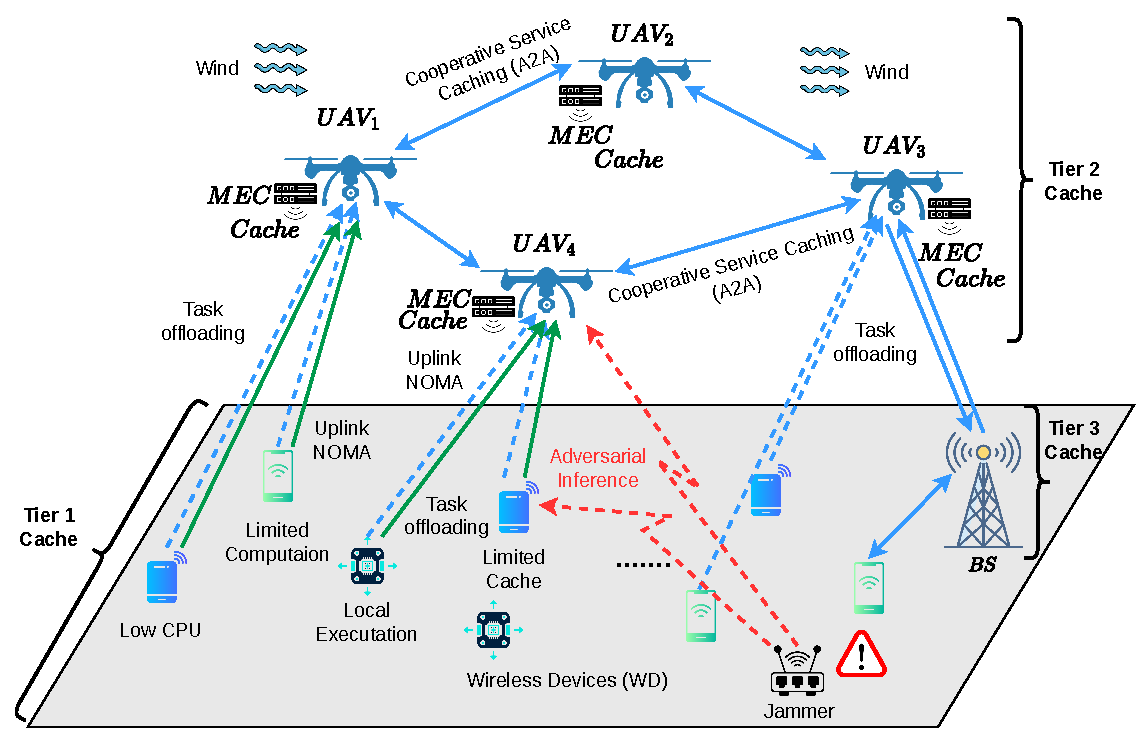
\includegraphics[width=0.8\linewidth]{images/service_caching_env.pdf}
  \caption{Proposed Multi UAV MEC Network}
  \label{fig:example}
\end{figure}


\section{System Model and Problem Formulation}
\label{section_III}
\subsection{Network Model}

In Fig \ref{fig:example}, we consider a UAV-enabled MEC-assisted IoT network operating over a finite horizon divided into $K$ decision epochs, indexed by $k\in\mathcal{K}\triangleq\{1,2,\dots,K\}$. The network consists of a set of mobile WDs, a set of MEC-enabled UAVs, one terrestrial BS, and a set of jammers. Let $\mathcal{N}\triangleq\{1,2,\dots,N\}$ denote the set of WDs. The position of WD $n\in\mathcal{N}$ at epoch $k$ is denoted by $\mathbf{w}_n(k)=[x_n(k),y_n(k),0]^\top$. Each WD has a local CPU frequency $f_n^{\mathrm{loc}}$ and limited cache capacity $C_n$, and may either execute a generated task locally or offload it to a UAV. Let $\mathcal{M}\triangleq\{1,2,\dots,M\}$ denote the set of UAVs. UAV $m\in\mathcal{M}$ flies in 3D with position
\begin{equation}
\mathbf{q}_m(k)=[x_m(k),y_m(k),h_m(k)]^\top,\quad 
h_m(k)\in[h_{\min},h_{\max}],
\end{equation}
where $h_{\min}$ and $h_{\max}$ are the minimum and maximum allowable flight altitudes, respectively. Each UAV is equipped with an onboard MEC server of CPU frequency $f_m^{\mathrm{uav}}$ and cache capacity $C_m^{\mathrm{uav}}$. UAVs execute offloaded tasks and cooperatively exchange cached service programs through A2A links when the required service is unavailable at the serving UAV. A single BS is deployed at $\mathbf{b}=[x_b,y_b,0]^\top$ and acts as a control anchor and complete service repository. It provides missing service programs to UAVs when the required service is unavailable in the serving UAV and cooperative UAV caches, but it does not participate in task computation. Thus, tasks are executed only at the originating WD or at a serving UAV, while the BS supports cache-miss service retrieval. The resulting service access structure consists of WD-level local caching, UAV-level cooperative caching, and BS-assisted service retrieval. Let $\mathcal{J}\triangleq\{1,2,\dots,J\}$ denote the set of jammers. Jammer $j\in\mathcal{J}$ is located at
$\mathbf{u}_j(k)=[x_j(k),y_j(k),0]^\top$
and transmits intentional interference to degrade WD-to-UAV uplink offloading links. The system evolves in epochs of duration $\Delta t$, and the mobility of WDs and UAVs is captured through $\{\mathbf{w}_n(k)\}$ and $\{\mathbf{q}_m(k)\}$.


\subsection{Mobility Model of WDs}

At the beginning of the mission horizon, all WDs are uniformly distributed within the monitoring region $\mathcal{A}$. The mobility of each WD $n\in\mathcal{N}$ is modeled using the Gauss-Markov (GM) model \cite{11395508}, which captures temporal correlation in both speed and heading direction. At each epoch $k\in\mathcal{K}$, the speed $v_n(k)$ and heading angle $\theta_n(k)$ evolve as
\begin{align}
    v_n(k) &= \rho_v v_n(k-1) + (1-\rho_v)\bar{v}_n 
              + \sqrt{1-\rho_v^2}\,\xi_n^v(k), \label{eq:gm_speed}\\
    \theta_n(k) &= \rho_\theta \theta_n(k-1) + (1-\rho_\theta)\bar{\theta}_n 
              + \sqrt{1-\rho_\theta^2}\,\xi_n^\theta(k), 
              \label{eq:gm_direction}
\end{align}
where $\bar{v}_n$ and $\bar{\theta}_n$ denote the mean speed and heading direction of WD $n$, respectively. The parameters $\rho_v,\rho_\theta\in[0,1]$ control the memory of the mobility process, while $\xi_n^v(k)\sim\mathcal{N}(0,\sigma_v^2)$ and $\xi_n^\theta(k)\sim\mathcal{N}(0,\sigma_\theta^2)$ are independent Gaussian perturbations. Based on the speed and heading at epoch $k-1$, the horizontal position of WD $n$ is updated as
\begin{align}
    x_n(k) &= x_n(k-1) + \Delta t\, v_n(k-1)\cos\theta_n(k-1), 
               \label{eq:pos_x}\\
    y_n(k) &= y_n(k-1) + \Delta t\, v_n(k-1)\sin\theta_n(k-1),
               \label{eq:pos_y}
\end{align}
such that $\mathbf{w}_n(k)=[x_n(k),y_n(k),0]^\top$. If the updated position moves outside $\mathcal{A}$, a specular reflection rule is applied to the heading direction to keep the WD trajectory within the monitoring region.

\subsection{Communication Model}
\subsubsection{Air-to-Ground Channel Model}

The primary offloading links between WDs and UAVs are modeled as 
probabilistic air-to-ground (A2G) channels, wherein the instantaneous propagation condition is either line-of-sight (LoS) or non-line-of-sight (NLoS) depending on the relative geometry and the surrounding environment 
\cite{11500527}. For WD $n\in\mathcal{N}$ and UAV $m\in\mathcal{M}$ at epoch 
$k$, the Euclidean distance is given by
\begin{equation}
\small
\begin{split}
    d_{n,m}(k)
    &= \left\|\mathbf{q}_m(k)-\mathbf{w}_n(k)\right\|_2 \\
    &= \sqrt{\bigl(x_m(k)-x_n(k)\bigr)^2
    + \bigl(y_m(k)-y_n(k)\bigr)^2
    + h_m^2(k)} ,
\end{split}
\label{eq:dist_wd_uav}
\end{equation}
and the corresponding elevation angle (in degrees) is $\phi_{n,m}(k)
    = \frac{180}{\pi}
    \arcsin\!\left(\frac{h_m(k)}{d_{n,m}(k)}\right).
\label{eq:elev_angle}$ The probability that the link between WN $n$ and UAV $m$ is LoS at epoch $k$ is expressed as
\begin{equation}
\small
    \mathcal{P}^{\mathrm{LoS}}_{n,m}(k)
    = \frac{1}{1+a\exp\!\left(-b\bigl(\phi_{n,m}(k)-a\bigr)\right)},
\label{eq:los_prob}
\end{equation}
where $a$ and $b$ are environment-dependent constants determined by the
propagation environment. The NLoS probability is then $\mathcal{P}^{\mathrm{NLoS}}_{n,m}(k)
    = 1-\mathcal{P}^{\mathrm{LoS}}_{n,m}(k).
\label{eq:nlos_prob}$

Let $\beta_{\mathrm{LoS}}$ and $\beta_{\mathrm{NLoS}}$ denote the
large-scale channel gain coefficients under LoS and NLoS propagation,
respectively, where $\beta_{\mathrm{LoS}}>\beta_{\mathrm{NLoS}}>0$.
Then, the corresponding LoS and NLoS channel gains are modeled as
\begin{align}
    g_{n,m}^{\mathrm{LoS}}(k)
    &= \beta_{\mathrm{LoS}}\bigl(d_{n,m}(k)\bigr)^{-\ell},
\label{eq:gain_los}\\
    g_{n,m}^{\mathrm{NLoS}}(k)
    &= \beta_{\mathrm{NLoS}}\bigl(d_{n,m}(k)\bigr)^{-\ell},
\label{eq:gain_nlos}
\end{align}
where $\ell$ denotes the path-loss exponent. Using the probability-weighted average large-scale channel model, the effective A2G channel gain between WN $n$ and UAV $m$ at epoch $k$ is given by
\begin{equation}
\small
\begin{split}
    g_{n,m}(k)
    &= \mathcal{P}^{\mathrm{LoS}}_{n,m}(k)\,
    g_{n,m}^{\mathrm{LoS}}(k)
    + \mathcal{P}^{\mathrm{NLoS}}_{n,m}(k)\,
    g_{n,m}^{\mathrm{NLoS}}(k) \\
    &= \Bigl[
    \mathcal{P}^{\mathrm{LoS}}_{n,m}(k)\beta_{\mathrm{LoS}}
    + \mathcal{P}^{\mathrm{NLoS}}_{n,m}(k)\beta_{\mathrm{NLoS}}
    \Bigr]
    \bigl(d_{n,m}(k)\bigr)^{-\ell}.
\end{split}
\label{eq:channel_gain_a2g}
\end{equation}

\subsubsection{Air-to-Air Channel Model}

Inter-UAV links are used only for cooperative caching exchange, where one
UAV may fetch a required service or cached content from another UAV. Due to the relatively high operating altitude of UAVs and the absence of significant aerial obstructions, inter-UAV links are assumed to
experience dominant LoS propagation. Therefore, the A2A channel gain between UAV $m$ and UAV $m'\in\mathcal{M}\setminus\{m\}$ at epoch $k$ is
modeled as \cite{8937764},
\begin{equation}
    g_{m,m'}(k)
    = \beta_{\mathrm{LoS}}
    \bigl(d_{m,m'}(k)\bigr)^{-\ell},
\label{eq:channel_gain_a2a}
\end{equation}
where $d_{m,m'}(k)
    = \left\|\mathbf{q}_m(k)-\mathbf{q}_{m'}(k)\right\|_2
\label{eq:dist_uav_uav}$ denotes the Euclidean distance between UAV $m$ and UAV $m'$.

\subsubsection{Jammer Interference Model}

Each jammer transmits fixed-power interference over the WD-to-UAV uplink spectrum. Since task offloading is the main wireless bottleneck, jamming is assumed to affect only WD-to-UAV links. For jammer $j\in\mathcal{J}$ and UAV $m$, the jammer-to-UAV distance is, $d_{j,m}(k)
    = \left\|\mathbf{q}_m(k)-\mathbf{u}_j(k)\right\|_2.
\label{eq:dist_jam_uav}$
The elevation angle is, $\phi_{j,m}(k)
    = \frac{180}{\pi}
    \arcsin\!\left(\frac{h_m(k)}{d_{j,m}(k)}\right).
\label{eq:elev_angle_jam}$
Using the same probabilistic A2G model, the jammer-to-UAV channel gain is
\begin{equation}
\small
    g_{j,m}(k)
    =
    \Bigl[
    \mathcal{P}^{\mathrm{LoS}}_{j,m}(k)\beta_{\mathrm{LoS}}
    + \mathcal{P}^{\mathrm{NLoS}}_{j,m}(k)\beta_{\mathrm{NLoS}}
    \Bigr]
    \bigl(d_{j,m}(k)\bigr)^{-\ell},
\label{eq:channel_gain_jam}
\end{equation}
where
\begin{equation}
\small
    \mathcal{P}^{\mathrm{LoS}}_{j,m}(k)
    = \frac{1}{1+a\exp\!\left(-b\bigl(\phi_{j,m}(k)-a\bigr)\right)}
\label{eq:los_prob_jam}
\end{equation}
and $\mathcal{P}^{\mathrm{NLoS}}_{j,m}(k)=1-\mathcal{P}^{\mathrm{LoS}}_{j,m}(k)$. Therefore, the aggregate jamming interference received at UAV $m$ is, $I_m(k)
    = \sum_{j\in\mathcal{J}} P_j^{\mathrm{jam}}\, g_{j,m}(k),
\label{eq:jam_agg}$
where $P_j^{\mathrm{jam}}$ is the transmit power of jammer $j$.

\subsubsection{NOMA-Based Uplink Transmission}

To enable simultaneous task offloading from multiple wireless nodes to
the same UAV, power-domain NOMA is adopted for the wireless
node-to-UAV uplink \cite{11020655}. Let $a_{n,m}(k)\in\{0,1\}$ denote the association
indicator, where $a_{n,m}(k)=1$ means that wireless node $n$ offloads
its task to UAV $m$ at epoch $k$, and $a_{n,m}(k)=0$ otherwise. Each wireless node can associate with at most one UAV at each epoch, i.e., $\sum_{m\in\mathcal{M}} a_{n,m}(k) \le 1,
    \quad \forall n\in\mathcal{N},\ \forall k\in\mathcal{K}. \label{eq:assoc_constraint}$
Let $\mathcal{N}_m(k)
    \triangleq \{n\in\mathcal{N}: a_{n,m}(k)=1\}
\label{eq:noma_cluster}$ denote the NOMA cluster served by UAV $m$ at epoch $k$. To ensure practical SIC complexity, the number of simultaneously served wireless nodes at each UAV is limited by $|\mathcal{N}_m(k)| \le N_m^{\max},
    \quad \forall m\in\mathcal{M},\ \forall k\in\mathcal{K},
\label{eq:noma_cluster_limit}$ where $N_m^{\max}$ is the maximum allowable NOMA cluster size of UAV $m$.

Let $p_n(k)$ denote the uplink transmit power of wireless node $n$ at
epoch $k$. Under uplink NOMA, UAV $m$ employs successive interference
cancellation (SIC) to decode the superimposed signals from all wireless
nodes in $\mathcal{N}_m(k)$. Assuming ideal SIC, previously decoded
signals are perfectly cancelled. The decoding order is determined by the
ascending order of effective channel gains, i.e., from the weakest to
the strongest channel. Let $\pi_m(k)$ denote the permutation over
$\mathcal{N}_m(k)$ such that, $g_{\pi_m^{(1)}(k),m}(k)
    \le g_{\pi_m^{(2)}(k),m}(k)
    \le \cdots
    \le g_{\pi_m^{(|\mathcal{N}_m(k)|)}(k),m}(k),
\label{eq:sic_order}$
where $\pi_m^{(i)}(k)$ is the WD decoded at the $i$-th SIC stage by UAV $m$. For a WD $n=\pi_m^{(i)}(k)$, the signals of nodes decoded in stages $1,\dots,i-1$ have already been removed, while the signals of
nodes decoded in stages $i+1,\dots,|\mathcal{N}_m(k)|$ remain as intra-cluster interference. Therefore, the received SINR of node
$n=\pi_m^{(i)}(k)$ at UAV $m$ is given by
\begin{equation}
\gamma_{n,m}(k)=
\textstyle\frac{p_n(k)g_{n,m}(k)}
{\sum_{r=i+1}^{|\mathcal{N}_m(k)|}p_{\pi_m^{(r)}(k)}(k)g_{\pi_m^{(r)}(k),m}(k)+I_m(k)+\sigma_0^2}.
\label{eq:sinr_noma}
\end{equation}
where $\sigma_0^2$ denotes the additive white Gaussian noise power at
the UAV receiver. Since different UAVs are assumed to operate on orthogonal resource
blocks, inter-cluster uplink interference among different UAVs is
ignored. Hence, the achievable uplink transmission rate of wireless node
$n$ offloading to UAV $m$ at epoch $k$ is
\begin{equation}
    R_{n,m}(k)
    = a_{n,m}(k)\, B
    \log_2\!\bigl(1+\gamma_{n,m}(k)\bigr),
\label{eq:rate_noma}
\end{equation}
where $B$ denotes the shared uplink bandwidth allocated to the NOMA
cluster served by UAV $m$. To guarantee offloading reliability, the achievable uplink rate must
satisfy the minimum QoS requirement of each wireless node, $R_{n,m}(k)
    \ge a_{n,m}(k)\, R_n^{\min},
    \quad \forall n\in\mathcal{N},\ \forall m\in\mathcal{M},\
    \forall k\in\mathcal{K}.
\label{eq:qos_constraint}$ Moreover, the uplink transmit power of each wireless node is constrained by, $0 \le p_n(k) \le P_n^{\max},
    \quad \forall n\in\mathcal{N},\ \forall k\in\mathcal{K}.
\label{eq:power_constraint}$

%==============================================================
\subsection{Three-Tier Service Caching and Availability Model}
\label{sec:caching_model}
%==============================================================

\subsubsection{Service Library and Popularity}

Let $\mathcal{L}\triangleq\{1,2,\dots,L\}$ denote the service library, where each service $l\in\mathcal{L}$ represents an application program required for task execution and occupies storage size $s_l$. Since service requests in MEC systems often follow a long-tail distribution, the request probability of service $l$ is modeled using a Zipf distribution, $p_l=\frac{l^{-\zeta}}{\sum_{i=1}^{L} i^{-\zeta}},\quad l\in\mathcal{L},
\label{eq:zipf}$
where services are indexed in descending order of popularity and $\zeta\geq0$ controls the skewness of the request distribution \cite{barman2025joint}.


\subsubsection{Three-Tier Service Caching States}

To reduce service access latency and improve execution flexibility, the proposed framework adopts a three-tier service availability architecture. At the first tier, WDs cache a limited number of service programs for local task execution. At the second tier, UAVs cache popular service programs and cooperatively share missing services through A2A links. At the third tier, the BS maintains the complete service library and provides missing service programs to UAVs when the requested service is unavailable in the cooperative 
UAV cache layer. The BS is not used for task computation; it only supports cache-miss service retrieval. Let $c_{n,l}(k)\in\{0,1\}$ and $c_{m,l}(k)\in\{0,1\}$ denote the caching state of service $l$ at WD $n$ and UAV $m$ during epoch $k$, respectively. These variables are defined as
\begin{equation}
\small
    c_{n,l}(k)=
    \begin{cases}
        1, & \text{if service } l \text{ is cached at WD } n 
        \text{ during epoch } k,\\
        0, & \text{otherwise},
    \end{cases}
    \label{eq:wd_cache_state}
\end{equation}
and
\begin{equation}
\small
    c_{m,l}(k)=
    \begin{cases}
        1, & \text{if service } l \text{ is cached at UAV } m 
        \text{ during epoch } k,\\
        0, & \text{otherwise}.
    \end{cases}
    \label{eq:uav_cache_state}
\end{equation}
Since WDs and UAVs have limited storage capacity, their caching decisions must satisfy $\sum_{l\in\mathcal{L}} c_{n,l}(k)s_l \leq C_n,
    \quad \forall n\in\mathcal{N},\;\forall k\in\mathcal{K},
    \label{eq:wd_cache_cap}$
and $\sum_{l\in\mathcal{L}} c_{m,l}(k)s_l \leq C_m^{\mathrm{uav}},
    \quad \forall m\in\mathcal{M},\;\forall k\in\mathcal{K},
    \label{eq:uav_cache_cap}$
where $C_n$ and $C_m^{\mathrm{uav}}$ denote the cache capacities of WD $n$ and UAV $m$, respectively. In general, $C_n\ll C_m^{\mathrm{uav}}$, reflecting the fact that WDs are resource-constrained, whereas UAVs 
are equipped with relatively larger onboard storage.

In addition, the BS is modeled as a complete service repository. Let $c_{b,l}$ denote the availability of service $l$ at the BS. Since the BS stores all services in the library, we have, $c_{b,l}=1,\quad \forall l\in\mathcal{L}.
    \label{eq:bs_cache_state}$
Unlike WDs and UAVs, the BS is assumed to have sufficient storage for the complete service library and is therefore not subject to a cache 
capacity constraint. However, retrieving a service from the BS incurs an additional BS-to-UAV service fetching delay.

\subsubsection{Cooperative Inter-UAV Service Fetching}

Due to finite UAV cache capacity, UAVs cooperatively share cached services through dedicated A2A links. If UAV $m$ serves WD $n$ but does not cache the required service $s_n(k)$, it may fetch the service from another UAV $m'\in\mathcal{M}\setminus\{m\}$ with $c_{m',s_n(k)}(k)=1$. These A2A links are used only for service fetching, not for relaying WD task data. The cooperative service fetch rate is
\begin{equation}
\small
    R_{m,m'}^{\mathrm{coop}}(k)=
    B^{\mathrm{A2A}}\log_2\!\left(
    1+\frac{P_{m'}^{\mathrm{uav}}g_{m,m'}(k)}{\sigma_0^2}
    \right),
    \label{eq:coop_rate}
\end{equation}
where $B^{\mathrm{A2A}}$, $P_{m'}^{\mathrm{uav}}$, and $g_{m,m'}(k)$ denote the A2A bandwidth, transmitting UAV power, and A2A channel gain, respectively.

\subsubsection{BS-Assisted Service Fetching}

If $s_n(k)$ is unavailable in the cooperative UAV cache layer, UAV $m$ retrieves it from the BS repository. The BS-to-UAV fetching rate is
\begin{equation}
\small
    R_{b,m}^{\mathrm{BS}}(k)=
    B^{\mathrm{BS}}\log_2\!\left(
    1+\frac{P_b g_{b,m}(k)}{\sigma_0^2}
    \right),
    \label{eq:bs_fetch_rate}
\end{equation}
where $B^{\mathrm{BS}}$, $P_b$, and $g_{b,m}(k)$ denote the BS-to-UAV bandwidth, BS transmit power, and BS-to-UAV channel gain, respectively. Let $\mathcal{M}_{m,l}^{\mathrm{coop}}(k)=
\{m'\in\mathcal{M}\setminus\{m\}\mid c_{m',l}(k)=1\}$ denote the set of UAVs caching service $l$. If $\mathcal{M}_{m,s_n(k)}^{\mathrm{coop}}(k)\neq\emptyset$, the service-providing UAV is selected as
$m^\star=\arg\max_{m'\in\mathcal{M}_{m,s_n(k)}^{\mathrm{coop}}(k)}
R_{m,m'}^{\mathrm{coop}}(k)$. Therefore, the service fetching delay is
\begin{equation}
\small
T_{n,m}^{\mathrm{fetch}}(k)=
\begin{cases}
0, 
& c_{m,s_n(k)}(k)=1,\\[1mm]
\dfrac{s_{s_n(k)}}{R_{m,m^\star}^{\mathrm{coop}}(k)}, 
& c_{m,s_n(k)}(k)=0,\;
\mathcal{M}_{m,s_n(k)}^{\mathrm{coop}}(k)\neq\emptyset,\\[3mm]
\dfrac{s_{s_n(k)}}{R_{b,m}^{\mathrm{BS}}(k)}, 
& c_{m,s_n(k)}(k)=0,\;
\mathcal{M}_{m,s_n(k)}^{\mathrm{coop}}(k)=\emptyset.
\end{cases}
\label{eq:fetch_delay}
\end{equation}
Thus, $T_{n,m}^{\mathrm{fetch}}(k)$ captures local UAV cache hits, A2A cooperative fetching, and BS-assisted cache-miss recovery.

\subsubsection{Effective Service Availability}

The cooperative UAV-level service availability indicator is defined as
\begin{equation}
\small
    \tilde{c}_{m,l}^{\mathrm{uav}}(k)=
    \begin{cases}
        1, & c_{m,l}(k)=1,\\
        1, & \exists\, m'\in\mathcal{M}\setminus\{m\}: c_{m',l}(k)=1,\\
        0, & \text{otherwise}.
    \end{cases}
    \label{eq:effective_uav_cache}
\end{equation}
Since the BS stores the complete service library, system-level service availability is $\tilde{c}_{m,l}^{\mathrm{sys}}(k)=1,
    \quad \forall m\in\mathcal{M},\;\forall l\in\mathcal{L},\;
    \forall k\in\mathcal{K}.
    \label{eq:effective_sys_cache}$
Here, $\tilde{c}_{m,l}^{\mathrm{uav}}(k)$ indicates low-latency UAV-level availability, whereas $\tilde{c}_{m,l}^{\mathrm{sys}}(k)$ guarantees service retrieval through BS-assisted fetching.

\subsubsection{Caching-Execution Feasibility}

Local execution at WD $n$ is feasible only when the required service is cached locally:
$x_n^{\mathrm{loc}}(k)\leq c_{n,s_n(k)}(k),\;\forall n,k. \label{local}$
For UAV-assisted execution, a UAV cache miss does not block offloading because the service can be retrieved through A2A fetching or from the BS repository. Hence, UAV offloading feasibility is governed by task assignment, NOMA cluster-size, QoS, and UAV resource constraints, while caching affects only $T_{n,m}^{\mathrm{fetch}}(k)$.


\subsection{Computation Model}
\label{sec:computation_model}

\subsubsection{Task Generation Model}

At each epoch $k\in\mathcal{K}$, WD $n\in\mathcal{N}$ generates a task with probability $p_0$. Let $\delta_n(k)\in\{0,1\}$ denote the task-generation indicator. A generated task is represented as
$T_n(k)=\bigl(D_n(k),F_n(k),s_n(k)\bigr)$, where $D_n(k)$ is the input data size, $F_n(k)$ is the required CPU cycles, and $s_n(k)\in\mathcal{L}$ is the required service type drawn according to Zipf popularity distribution \eqref{eq:zipf}.


\subsubsection{Execution Assignment}

Each generated task is executed either locally at its originating WD or remotely at one serving UAV; the BS only provides missing services and does not execute tasks. Let $x_n^{\mathrm{loc}}(k)\in\{0,1\}$ and $a_{n,m}(k)\in\{0,1\}$ denote the local execution and UAV offloading indicators, respectively. The assignment constraint is
\begin{equation}
\small
    x_n^{\mathrm{loc}}(k)+\sum_{m\in\mathcal{M}}a_{n,m}(k)
    = \delta_n(k),
    \quad \forall n\in\mathcal{N},\;\forall k\in\mathcal{K}.
    \label{eq:exec_assign}
\end{equation}
Local execution must satisfy \eqref{local}, while UAV execution remains feasible under cache misses because the required service can be retrieved through A2A fetching or BS-assisted retrieval.

\subsubsection{Local Computation Delay}

If $x_n^{\mathrm{loc}}(k)=1$, task $T_n(k)$ is executed at WD $n$ with CPU frequency $f_n^{\mathrm{loc}}$, and the local delay is
\begin{equation}
\small
    T_n^{\mathrm{loc}}(k)=\frac{F_n(k)}{f_n^{\mathrm{loc}}},
    \quad \forall n\in\mathcal{N},\;\forall k\in\mathcal{K}.
    \label{eq:local_delay}
\end{equation}

\subsubsection{UAV Offloading Delay}

If $a_{n,m}(k)=1$, task $T_n(k)$ is offloaded to UAV $m$, and the completion delay includes uplink transmission, service fetching, queue waiting, and UAV computation delays. The uplink transmission delay is
\begin{equation}
\small
    T_{n,m}^{\mathrm{tx}}(k)=\frac{D_n(k)}{R_{n,m}(k)}.
    \label{eq:tx_delay}
\end{equation}
The service fetching delay $T_{n,m}^{\mathrm{fetch}}(k)$ follows the three-tier availability model in \eqref{eq:fetch_delay}. Each UAV maintains a FIFO computation queue. Let $Z_m(k)$ denote the queued workload at UAV $m$ in CPU cycles. Its evolution is
\begin{equation}
\small
Z_m(k+1)=
\max\left\{
Z_m(k)+\sum_{n\in\mathcal{N}}a_{n,m}(k)\delta_n(k)F_n(k)
-f_m^{\mathrm{uav}}\Delta t,\;0
\right\}.
\label{eq:queue_update}
\end{equation}
The corresponding queue waiting delay is
\begin{equation}
\small
Q_m(k)=\frac{Z_m(k)}{f_m^{\mathrm{uav}}}.
\label{eq:queue_delay}
\end{equation}
After data and service availability, UAV $m$ executes the task with computation delay
\begin{equation}
\small
    T_{n,m}^{\mathrm{cmp}}(k)=\frac{F_n(k)}{f_m^{\mathrm{uav}}}.
    \label{eq:uav_cmp_delay}
\end{equation}
Thus, the total UAV-side task completion delay is
\begin{equation}
\small
    T_{n,m}^{\mathrm{uav}}(k)
    = T_{n,m}^{\mathrm{tx}}(k)
    + T_{n,m}^{\mathrm{fetch}}(k)
    + Q_m(k)
    + T_{n,m}^{\mathrm{cmp}}(k).
    \label{eq:total_uav_delay}
\end{equation}

\subsubsection{Unified Task Completion Delay}

The total task completion delay of WD $n$ at epoch $k$ is
\begin{equation}
\small
    T_n^{\mathrm{tot}}(k)
    = x_n^{\mathrm{loc}}(k)T_n^{\mathrm{loc}}(k)
    + \sum_{m\in\mathcal{M}} a_{n,m}(k)T_{n,m}^{\mathrm{uav}}(k),
    \label{eq:total_delay}
\end{equation}
which becomes zero when $\delta_n(k)=0$ due to \eqref{eq:exec_assign}. The average task completion delay over all generated tasks is
\begin{equation}
\small
    \bar{T}=
    \frac{\sum_{k\in\mathcal{K}}\sum_{n\in\mathcal{N}}
    \delta_n(k)T_n^{\mathrm{tot}}(k)}
    {\sum_{k\in\mathcal{K}}\sum_{n\in\mathcal{N}}\delta_n(k)}.
    \label{eq:avg_delay}
\end{equation}


\subsection{Energy Consumption Model}
\label{sec:energy_model}

The total system energy includes WD local computation, WD uplink transmission, UAV computation, UAV cooperative service-fetching communication, and UAV propulsion energy:
\begin{equation}
\small
    E^{\mathrm{total}}
    = \sum_{n\in\mathcal{N}}
    \bigl(E_n^{\mathrm{loc}} + E_n^{\mathrm{tx}}\bigr)
    + \sum_{m\in\mathcal{M}}
    \bigl(E_m^{\mathrm{cmp}} + E_m^{\mathrm{comm}} + E_m^{\mathrm{fly}}\bigr).
    \label{eq:total_energy}
\end{equation}

\subsubsection{WD Energy Consumption}

Following the dynamic voltage and frequency scaling (DVFS) model, the local computation energy of WD $n$ is
\begin{equation}
\small
    E_n^{\mathrm{loc}}
    =
    \sum_{k\in\mathcal{K}}
    x_n^{\mathrm{loc}}(k)\delta_n(k)
    \kappa_n \bigl(f_n^{\mathrm{loc}}\bigr)^2 F_n(k),
    \label{eq:wd_loc_energy_total}
\end{equation}
where $\kappa_n$ and $f_n^{\mathrm{loc}}$ denote the effective switched capacitance and local CPU frequency, respectively. The uplink transmission energy is
\begin{equation}
\small
    E_n^{\mathrm{tx}}
    =
    \sum_{k\in\mathcal{K}}\sum_{m\in\mathcal{M}}
    a_{n,m}(k)\delta_n(k)
    \frac{p_n(k)D_n(k)}{R_{n,m}(k)}.
    \label{eq:wd_tx_energy_total}
\end{equation}

\subsubsection{UAV Energy Consumption}

The energy consumed by UAV $m$ is
\begin{equation}
\small
    E_m^{\mathrm{total}}
    = E_m^{\mathrm{cmp}} + E_m^{\mathrm{comm}} + E_m^{\mathrm{fly}}.
    \label{eq:uav_total_energy}
\end{equation}
The onboard computation energy is
\begin{equation}
\small
    E_m^{\mathrm{cmp}}
    =
    \sum_{k\in\mathcal{K}}\sum_{n\in\mathcal{N}}
    a_{n,m}(k)\delta_n(k)
    \kappa_m \bigl(f_m^{\mathrm{uav}}\bigr)^2 F_n(k),
    \label{eq:uav_cmp_energy_total}
\end{equation}
where $\kappa_m$ and $f_m^{\mathrm{uav}}$ are the UAV capacitance coefficient and CPU frequency.

Let $y_{n,m,m'}(k)\in\{0,1\}$ indicate whether UAV $m'$ sends the required service of task $T_n(k)$ to serving UAV $m$. The cooperative service-fetching communication energy of UAV $m'$ is
\begin{equation}
\small
    E_{m'}^{\mathrm{comm}}
    =
    \sum_{k\in\mathcal{K}}
    \sum_{n\in\mathcal{N}}
    \sum_{\substack{m\in\mathcal{M}\\ m\neq m'}}
    y_{n,m,m'}(k)P_{m'}^{\mathrm{uav}}
    T_{n,m}^{\mathrm{fetch}}(k).
    \label{eq:uav_comm_energy_total}
\end{equation}
The BS is assumed grid-powered; hence, its service-retrieval energy is not included in the UAV energy budget.

For rotary-wing UAVs, the propulsion power at speed $v_m(k)$ is modeled as \cite{11500527}
\begin{equation}
\small
\begin{split}
    P_m^{\mathrm{fly}}(k)
    &= \eta_1\!\left(1+\frac{3v_m^2(k)}{v_{\mathrm{tip}}^2}\right)
    + \eta_2\!\left(\sqrt{\eta_3+\frac{v_m^4(k)}{4}}
    - \frac{v_m^2(k)}{2}\right)^{\frac{1}{2}} \\
    &\quad + \eta_4 v_m^3(k),
    \label{eq:uav_prop_power}
\end{split}
\end{equation}
where $v_{\mathrm{tip}}$ and $\eta_1,\eta_2,\eta_3,\eta_4$ are aerodynamic constants, and 
$v_m(k)=\frac{\|\mathbf{q}_m(k+1)-\mathbf{q}_m(k)\|_2}{\Delta t}$.
The total propulsion energy is
\begin{equation}
\small
    E_m^{\mathrm{fly}}
    = \Delta t \sum_{k=1}^{K-1} P_m^{\mathrm{fly}}(k).
    \label{eq:uav_fly_energy_total}
\end{equation}
Finally, the UAV energy budget is
\begin{equation}
\small
    E_m^{\mathrm{cmp}} + E_m^{\mathrm{comm}} + E_m^{\mathrm{fly}}
    \leq E_m^{\max},
    \quad \forall m\in\mathcal{M}.
    \label{eq:uav_energy_budget}
\end{equation}










% The total energy consumption in the proposed multi-UAV-assisted MEC 
% system originates from three major sources: i) local computation and 
% uplink task transmission at the wireless devices (WDs), ii) onboard 
% computation and cooperative inter-UAV service fetching at the UAVs, 
% and iii) propulsion energy consumed during UAV flight. Accordingly, 
% the total energy consumption over the mission horizon can be expressed as
% \begin{equation}
%     E^{\mathrm{total}}
%     = \sum_{n\in\mathcal{N}}
%     \Bigl(E_n^{\mathrm{loc}} + E_n^{\mathrm{tx}}\Bigr)
%     + \sum_{m\in\mathcal{M}}
%     \Bigl(E_m^{\mathrm{cmp}} + E_m^{\mathrm{comm}} + E_m^{\mathrm{fly}}\Bigr),
%     \label{eq:total_energy}
% \end{equation}
% where the first summation captures the energy consumed by all WDs, 
% whereas the second summation represents the energy expenditure of all 
% UAVs.

% \subsubsection{WD Energy Consumption}

% Each WD consumes energy through two possible activities: local task 
% execution and wireless uplink transmission.

% \textbf{(i) Local Computation Energy:}  
% When WD $n$ executes task $T_n(k)$ locally, the corresponding energy 
% consumption follows the standard dynamic voltage and frequency scaling 
% (DVFS) model, under which the computation energy depends on the square 
% of the operating CPU frequency and the total number of CPU cycles. 
% Thus, the local computation energy of WD $n$ at epoch $k$ is given by
% \begin{equation}
%     E_{n,k}^{\mathrm{loc}}
%     = \kappa_n \bigl(f_n^{\mathrm{loc}}\bigr)^2 F_n(k),
%     \label{eq:wd_loc_energy}
% \end{equation}
% where $\kappa_n$ denotes the effective switched capacitance coefficient 
% of the processor of WD $n$, and $f_n^{\mathrm{loc}}$ is its local CPU 
% frequency. Therefore, the aggregate local computation energy of WD $n$ 
% over the mission horizon is
% \begin{equation}
%     E_n^{\mathrm{loc}}
%     = \sum_{k\in\mathcal{K}}
%     x_n^{\mathrm{loc}}(k)\,\delta_n(k)\,E_{n,k}^{\mathrm{loc}}.
%     \label{eq:wd_loc_energy_total}
% \end{equation}

% \textbf{(ii) Uplink Transmission Energy:}  
% When WD $n$ offloads its generated task to UAV $m$, it transmits the 
% input data $D_n(k)$ over the uplink channel with transmit power 
% $p_n(k)$. Since the uplink transmission duration equals 
% $T_{n,m}^{\mathrm{tx}}(k)=D_n(k)/R_{n,m}(k)$, the corresponding 
% transmission energy is
% \begin{equation}
%     E_{n,m,k}^{\mathrm{tx}}
%     = p_n(k)\,T_{n,m}^{\mathrm{tx}}(k)
%     = \frac{p_n(k)\,D_n(k)}{R_{n,m}(k)},
%     \label{eq:wd_tx_energy}
% \end{equation}
% where $R_{n,m}(k)$ is the achievable uplink transmission rate defined 
% in the communication model. Accordingly, the total uplink transmission 
% energy consumed by WD $n$ over all epochs is
% \begin{equation}
%     E_n^{\mathrm{tx}}
%     = \sum_{k\in\mathcal{K}}\sum_{m\in\mathcal{M}}
%     a_{n,m}(k)\,\delta_n(k)\,E_{n,m,k}^{\mathrm{tx}}.
%     \label{eq:wd_tx_energy_total}
% \end{equation}

% \subsubsection{UAV Energy Consumption}

% Each UAV consumes energy through onboard task computation, cooperative 
% inter-UAV service transmission, and flight propulsion. Thus, the total 
% energy consumed by UAV $m$ over the mission horizon is
% \begin{equation}
%     E_m^{\mathrm{total}}
%     = E_m^{\mathrm{cmp}} + E_m^{\mathrm{comm}} + E_m^{\mathrm{fly}},
%     \label{eq:uav_total_energy}
% \end{equation}
% where the three terms correspond to computation energy, cooperative 
% communication energy, and propulsion energy, respectively.

% \textbf{(i) Onboard Computation Energy:}  
% When UAV $m$ executes the offloaded task $T_n(k)$, its onboard MEC 
% processor consumes energy according to the DVFS model. The computation 
% energy required for processing task $T_n(k)$ at UAV $m$ is therefore
% \begin{equation}
%     E_{n,m,k}^{\mathrm{cmp}}
%     = \kappa_m \bigl(f_m^{\mathrm{uav}}\bigr)^2 F_n(k),
%     \label{eq:uav_cmp_energy}
% \end{equation}
% where $\kappa_m$ is the effective switched capacitance coefficient of 
% the processor of UAV $m$, and $f_m^{\mathrm{uav}}$ denotes its CPU 
% frequency. Summing over all tasks processed by UAV $m$, the total 
% onboard computation energy is
% \begin{equation}
%     E_m^{\mathrm{cmp}}
%     = \sum_{k\in\mathcal{K}}\sum_{n\in\mathcal{N}}
%     a_{n,m}(k)\,\delta_n(k)\,E_{n,m,k}^{\mathrm{cmp}}.
%     \label{eq:uav_cmp_energy_total}
% \end{equation}

% \textbf{(ii) Cooperative Communication Energy:}  
% In the proposed framework, inter-UAV communication is used exclusively 
% for cooperative service fetching. To explicitly indicate whether the 
% required service of task $T_n(k)$ is fetched by serving UAV $m$ from 
% another UAV $m'$, we define a binary fetch indicator, $y_{n,m,m'}(k)\in\{0,1\},
%     \label{eq:fetch_indicator}$
% where $y_{n,m,m'}(k)=1$ means that the required service of task $T_n(k)$ is transmitted from UAV $m'$ to UAV $m$ at epoch $k$, and $y_{n,m,m'}(k)=0$ otherwise. When such a fetching event occurs, UAV $m'$ transmits the required service to UAV $m$ over the A2A link with transmit power $P_{m'}^{\mathrm{uav}}$ for a duration equal to the service fetching delay $T_{n,m}^{\mathrm{fetch}}(k)$. Therefore, the corresponding cooperative communication energy is
% \begin{equation}
%     E_{n,m,m',k}^{\mathrm{comm}}
%     = y_{n,m,m'}(k)\,P_{m'}^{\mathrm{uav}}\,
%     T_{n,m}^{\mathrm{fetch}}(k).
%     \label{eq:uav_comm_energy}
% \end{equation}
% The total cooperative communication energy consumed by UAV $m'$ over 
% the mission horizon is then given by
% \begin{equation}
%     E_{m'}^{\mathrm{comm}}
%     = \sum_{k\in\mathcal{K}}
%     \sum_{n\in\mathcal{N}}
%     \sum_{\substack{m\in\mathcal{M}\\ m\neq m'}}
%     E_{n,m,m',k}^{\mathrm{comm}}.
%     \label{eq:uav_comm_energy_total}
% \end{equation}

% \textbf{(iii) Propulsion Energy:}  
% The propulsion energy is typically the dominant component of UAV energy 
% consumption and depends strongly on the UAV trajectory. For a rotary-wing 
% UAV, the instantaneous propulsion power of UAV $m$ flying at speed 
% $v_m(k)$ is modeled as
% \begin{equation}
% \begin{split}
%     P_m^{\mathrm{fly}}(k)
%     &= \underbrace{\eta_1\!\left(1+\frac{3v_m^2(k)}{v_{\mathrm{tip}}^2}\right)}_{\text{blade profile}}
%     + \underbrace{\eta_2\!\left(\sqrt{\eta_3+\frac{v_m^4(k)}{4}}
%     - \frac{v_m^2(k)}{2}\right)^{\frac{1}{2}}}_{\text{induced}} \\
%     &\quad + \underbrace{\eta_4 v_m^3(k)}_{\text{parasite}},
%     \label{eq:uav_prop_power}
% \end{split}
% \end{equation}
% where $v_{\mathrm{tip}}$ denotes the rotor blade tip speed, and 
% $\eta_1,\eta_2,\eta_3,\eta_4$ are UAV-dependent constants determined by 
% its physical and aerodynamic parameters. The three terms in 
% \eqref{eq:uav_prop_power} respectively represent the blade profile 
% power, the induced power, and the parasite power. The instantaneous flight speed of UAV $m$ during epoch $k$ is given by, $v_m(k) = \frac{\left\|\mathbf{q}_m(k+1)-\mathbf{q}_m(k)\right\|_2}{\Delta t},
% \quad \forall m\in\mathcal{M},\; k=1,\dots,K-1,
% \label{eq:uav_speed}$ which must satisfy the UAV speed constraint, $v_m(k)\leq v_m^{\max}, \quad \forall m\in\mathcal{M},\; k=1,\dots,K-1.
% \label{eq:uav_speed_constraint}$ Since the duration of each epoch is $\Delta t$, the propulsion energy consumed by UAV $m$ during epoch $k$ equals 
% $P_m^{\mathrm{fly}}(k)\Delta t$. Therefore, the total propulsion energy 
% over the mission horizon is
% \begin{equation}
%     E_m^{\mathrm{fly}}
%     = \Delta t \sum_{k=1}^{K-1} P_m^{\mathrm{fly}}(k).
%     \label{eq:uav_fly_energy_total}
% \end{equation}
% Finally, the total energy consumed by each UAV during the mission must 
% not exceed its onboard battery capacity. Thus, the UAV energy budget 
% constraint is
% \begin{equation}
%     E_m^{\mathrm{cmp}} + E_m^{\mathrm{comm}} + E_m^{\mathrm{fly}}
%     \leq E_m^{\max},
%     \quad \forall m\in\mathcal{M},
%     \label{eq:uav_energy_budget}
% \end{equation}
% where $E_m^{\max}$ denotes the maximum available energy of UAV $m$.


\subsection{Problem Formulation}
The objective is to minimize the average task completion latency while regularizing UAV energy consumption through joint optimization of UAV trajectory, task offloading, transmission power, and service caching decisions. Due to binary offloading/caching variables, continuous trajectory/power variables, and nonlinear coupling among communication, computation, service fetching, and energy models, the problem is formulated as a stochastic mixed-integer non-linear 
programming (MINLP). The optimization problem is formulated as follows:

\begin{equation}
\small
\begin{aligned}
\min_{X} \;\; 
& \frac{1}{\sum_{k\in\mathcal{K}}\sum_{n\in\mathcal{N}}\delta_n(k)}
\sum_{k\in\mathcal{K}}\sum_{n\in\mathcal{N}}
\delta_n(k)\,T_n^{\mathrm{tot}}(k) \\
& + \mu \sum_{k\in\mathcal{K}}\sum_{m\in\mathcal{M}}
E_m^{\mathrm{total}}(k)
\end{aligned}
\label{eq:problem_obj}
\end{equation}
where $\mu \geq 0$ is a non-negative weighting coefficient that controls the trade-off between latency and energy consumption, 
$X=\{\mathbf{q}_m(k),\,a_{n,m}(k),\,x_n^{\mathrm{loc}}(k),
\,p_n(k),\,c_{n,l}(k),\,c_{m,l}(k)\}$ represents the set of optimization 
variables, and $T_n^{\mathrm{tot}}(k)$ denotes the total task completion 
delay. The total UAV energy consumption is given by 
$E_m^{\mathrm{total}}(k)=E_m^{\mathrm{cmp}}(k)+E_m^{\mathrm{comm}}(k)
+E_m^{\mathrm{fly}}(k)$.

\begin{align}
&\mathcal{C}_1:\quad
x_n^{\mathrm{loc}}(k) + \sum_{m\in\mathcal{M}} a_{n,m}(k)
= \delta_n(k),
&& \forall n,k
\label{eq:c1}\\
&\mathcal{C}_2:\quad
x_n^{\mathrm{loc}}(k) \leq c_{n,s_n(k)}(k),
&& \forall n,k
\label{eq:c2}\\
&\mathcal{C}_3:\quad
\sum_{l\in\mathcal{L}} c_{n,l}(k)\,s_l \leq C_n,
&& \forall n,k
\label{eq:c3}\\
&\mathcal{C}_4:\quad
\sum_{l\in\mathcal{L}} c_{m,l}(k)\,s_l \leq C_m^{\mathrm{uav}},
&& \forall m,k
\label{eq:c4}\\
&\mathcal{C}_5:\quad
0 \leq p_n(k) \leq p_n^{\max},
&& \forall n,k
\label{eq:c5}\\
&\mathcal{C}_6:\quad
\|\mathbf{q}_m(k+1)-\mathbf{q}_m(k)\|
\le v_m^{\max}\Delta t,
&& \forall m,k
\label{eq:c6}\\
&\mathcal{C}_7:\quad
h_{\min}\le h_m(k)\le h_{\max},
&& \forall m,k
\label{eq:c7}\\
&\mathcal{C}_8:\quad
E_m^{\mathrm{cmp}} + E_m^{\mathrm{comm}} + E_m^{\mathrm{fly}}
\leq E_m^{\max},
&& \forall m
\label{eq:c8}\\
&\mathcal{C}_9:\quad
\mathbf{q}_m(k)\in\mathcal{A},
&& \forall m,k
\label{eq:c9}\\
&\mathcal{C}_{10}:\quad
|\mathcal{N}_m(k)| \le N_m^{\max},
&& \forall m,k
\label{eq:c10}\\
&\mathcal{C}_{11}:\quad
R_{n,m}(k) \ge a_{n,m}(k)\,R_n^{\min},
&& \forall n,m,k
\label{eq:c11}
\end{align}

Constraint $\mathcal{C}_1$ enforces unique task assignment, while $\mathcal{C}_2$ ensures WD-cache feasibility for local execution. Since the BS stores the complete service library, UAV cache misses affect $T_{n,m}^{\mathrm{fetch}}(k)$ rather than blocking UAV offloading. Constraints $\mathcal{C}_3$--$\mathcal{C}_5$ impose cache and transmit-power limits. Constraints $\mathcal{C}_6$--$\mathcal{C}_9$ define UAV mobility, altitude, energy, and deployment-region constraints. Finally, $\mathcal{C}_{10}$ and $\mathcal{C}_{11}$ enforce NOMA cluster-size and QoS requirements, respectively.

\section{Proposed Methodology}
\label{section_IV}
\subsection{Overall Framework for Joint Optimization}

The formulated problem involves hybrid decision variables, stochastic system dynamics, and strong coupling among task offloading, cooperative caching, NOMA-based resource allocation, UAV trajectory, and jammer-induced interference. These couplings make the stochastic MINLP difficult to solve directly using conventional optimization methods. In particular, caching affects service availability and service-fetching delay, offloading determines traffic distribution and NOMA interference, and UAV mobility changes channel quality, jamming exposure, and propulsion energy consumption. To address these challenges, we propose the \textit{Diffusion-based Multi-UAV Joint Optimization (DMJO)} framework. DMJO decomposes the original problem into four tightly coupled modules: (i) adaptive cooperative caching for service placement, (ii) MAPPO-based UAV trajectory control, (iii) diffusion-enhanced DRL for combinatorial task offloading, and (iv) analytical NOMA-based power allocation. These modules are jointly coordinated through a hierarchical learning framework to minimize task completion latency while regularizing UAV energy consumption.

To capture the different update rates of physical mobility, caching, and offloading decisions, DMJO adopts a \textit{two-timescale hierarchical framework}. The mission horizon is divided into macro-intervals and micro-epochs:
\begin{itemize}
    \item \textbf{Macro-timescale:} UAV trajectory and cooperative caching decisions are updated periodically and kept fixed within each macro-interval, since mobility adjustment and service replacement introduce physical and communication overhead.
    \item \textbf{Micro-timescale:} Given the macro-level trajectory and caching states, diffusion-enhanced task offloading and analytical NOMA power allocation are performed at each epoch to respond to stochastic task arrivals, time-varying channels, and jammer interference.
\end{itemize}
The learning modules operate under a CTDE paradigm. During offline training, a centralized critic uses global system information to guide policy learning, while during online execution, each UAV makes real-time decisions using only local observations and the learned policies. This design enables scalable multi-UAV coordination in dynamic jammer-aware MEC-IoT networks.



% The formulated problem involves hybrid decision variables, stochastic system dynamics, and strong coupling among task offloading, cooperative caching, NOMA-based resource allocation, and UAV trajectory design. It can therefore be modeled as a stochastic mixed-integer non-linear programming (MINLP) problem, which is computationally intractable to solve directly using conventional solvers.

% The key challenge lies in the interdependence among system components. Caching affects service availability and execution delay, directly influencing offloading feasibility; offloading decisions determine traffic distribution and influence interference patterns in the NOMA uplink; and UAV mobility dictates the spatial channel conditions and exposure to adversarial jamming, while also impacting propulsion energy consumption. These highly coupled interactions necessitate a unified optimization framework.

% To address this, we propose the \textit{Diffusion-based Multi-UAV Joint Optimization (DMJO)} framework. DMJO adopts a hierarchical decomposition approach that partitions the problem into four interdependent modules: (i) adaptive cooperative caching for service placement, (ii) Multi-Agent Proximal Policy Optimization (MAPPO) for UAV trajectory and control, (iii) diffusion-enhanced Deep Reinforcement Learning (DRL) for combinatorial task offloading, and (iv) analytical NOMA-based power allocation for communication. These modules are tightly coupled and jointly optimized through a hierarchical learning framework, enabling the joint optimization of task completion latency and UAV energy consumption.

% To reconcile the physical kinematic limits of UAVs with the necessity for ultra-low latency computation, we propose a \textit{two-timescale hierarchical framework}. While prior works such as TJCCT \cite{TJCCT} have explored timescale separation using conventional approximations, DMJO uniquely integrates deep generative models to scale across high-dimensional hybrid spaces. The mission horizon is decoupled into macro-intervals and micro-epochs:
% \begin{itemize}
%     \item \textbf{Macro-Timescale (Intervals):} UAV trajectory updates and cooperative caching decisions are executed. Because altering physical flight paths and fetching large service programs over inter-UAV backhaul links incur significant physical and temporal overhead, these variables are updated periodically and held constant over the duration of the macro-interval.
%     \item \textbf{Micro-Timescale (Epochs):} Operating within the spatial and service boundary conditions set by the macro-interval, diffusion-enhanced task offloading decisions are executed at fine-grained time resolution, while NOMA transmission employs analytical power allocation (e.g., bisection-based optimization). This enables the system to react rapidly to stochastic task arrivals and time-varying channel conditions.
% \end{itemize}

% Furthermore, the learning-based modules operate under a Centralized Training with Decentralized Execution (CTDE) paradigm. During offline training, a centralized critic evaluates the global system state to guide policy updates. During online execution, the UAVs utilize the converged MAPPO and diffusion-enhanced policies to make real-time decisions based strictly on local observations. Overall, this hierarchical design provides a physically realistic, scalable, and unified solution for jammer-aware multi-UAV IoT networks.


\subsection{Hierarchical MDP Formulation}

To solve the stochastic MINLP, we model the system as a Hierarchical Markov Decision Process (HMDP). The system operates over macro-intervals indexed by $t$ with duration $\Delta T_c=K_c\Delta t$, where UAV trajectory and caching decisions are updated, and micro-epochs indexed by $k$, where task offloading and communication decisions are performed.

\subsubsection{State Space and Local Observations}

\begin{align}
\small
\mathcal{S}(k)=\{&
\mathbf{w}_n(k),\mathbf{q}_m(k),g_{n,m}(k),I_m(k),Q_m(k),
c_{n,l}(k), \nonumber\\
&c_{m,l}(k),D_n(k),F_n(k),s_n(k),\delta_n(k)\},
\quad \forall n,m,l .
\end{align}
This state captures network geometry, channel conditions, queue states, caching states, and task characteristics. During centralized training, the critic observes $\mathcal{S}(k)$, whereas during decentralized execution, UAV $m$ acts based on its local observation $o_m(tK_c)\subset\mathcal{S}(tK_c)$, including local channels, queue status, residual energy, and relative distances to nearby WDs and jammers.

\subsubsection{Hierarchical Action Space}

The learning-based action space is divided according to the decision timescale. At the macro-timescale, MAPPO outputs the UAV velocity actions:
\begin{equation}
\small
\mathcal{A}_{\mathrm{macro}}(t)=\{\mathbf{v}_m(tK_c)\}_{m\in\mathcal{M}},
\end{equation}
where $\mathbf{v}_m(tK_c)=[v_m^x(tK_c),v_m^y(tK_c),v_m^h(tK_c)]^\top$ controls horizontal and vertical UAV movement.

At the micro-timescale, the diffusion-enhanced actor generates offloading decisions:
\begin{equation}
\small
\mathcal{A}_{\mathrm{micro}}(k)
=
\{a_{n,m}(k),x_n^{\mathrm{loc}}(k)\}_{n\in\mathcal{N},m\in\mathcal{M}}.
\end{equation}
The caching states $\{c_{m,l}(tK_c)\}$ are updated by the adaptive caching module, while the transmit powers are obtained analytically through NOMA-based optimization and are not included in the RL action space.

\subsubsection{State Transition}

The transition from $\mathcal{S}(k)$ to $\mathcal{S}(k+1)$ follows the selected actions and physical dynamics. WD mobility follows the Gauss-Markov model, while UAV positions evolve at the macro-timescale as
\begin{equation}
\small
\mathbf{q}_m(k+K_c)=\mathbf{q}_m(k)+\mathbf{v}_m(tK_c)\Delta T_c .
\end{equation}
The updated UAV positions affect channel gains, jammer interference, service coverage, and queue evolution, while caching states remain fixed within each macro-interval.

\subsubsection{Reward Function}
To align with \eqref{eq:problem_obj}, the reward is defined as
\begin{equation}
    r(k) = \tfrac{1}{2}\,r^{\mathrm{global}}(k)
           + \tfrac{1}{2}\sum_{m\in\mathcal{M}} r_m^{\mathrm{shaped}}(k),
    \label{eq:reward}
\end{equation}
where
\begin{equation}
    r^{\mathrm{global}}(k)
    = -\alpha_L\!\left(\bar{T}(k) - \frac{N}{2M}\right)
      - \frac{\beta_E}{10^3}
        \sum_{m\in\mathcal{M}} E_m^{\mathrm{total}}(k),
    \label{eq:reward_global}
\end{equation}
with $(\alpha_L,\beta_E){=}(0.6,0.4)$ from \eqref{eq:problem_obj}.
The shaping term $r_m^{\mathrm{shaped}}(k)$ adds per-task outcome
rewards and penalises UAV collisions and boundary violations.

\subsubsection{Objective}

The objective of the HMDP is to learn an optimal joint policy $\pi^* = \{\pi_\phi^*, \pi_{\theta_m}^*\}$ that maximizes the expected cumulative discounted reward:
\begin{equation}
\small
\pi^* = \arg\max_{\pi} \mathbb{E}_{\tau \sim \pi} \left[ \sum_{k=1}^{K} \gamma^{k-1} r(k) \right],
\end{equation}
where $\gamma \in (0,1]$ is the discount factor and $\tau$ denotes the trajectory of states and actions.

\subsection{Cooperative Caching Module}

The caching module updates service placement at the macro-timescale to improve UAV-level service availability and reduce service retrieval delay. As defined in Section~\ref{sec:caching_model}, $c_{n,l}(k)$ and $c_{m,l}(k)$ denote WD and UAV cache states, respectively, while $\tilde{c}_{m,l}^{\mathrm{uav}}(k)$ captures whether service $l$ is available at UAV $m$ either locally or through A2A cooperative fetching. BS-assisted retrieval guarantees system-level service availability but introduces additional fetching delay.

\subsubsection{Adaptive Cooperative Caching Objective}

Each service $l$ is assigned a priority score based on request frequency and successful task completion:
\begin{equation}
\small
S_l(k)=
\lambda_f
\frac{N_l(k)}{\sum_{l'\in\mathcal{L}}N_{l'}(k)+\varepsilon}
+
\lambda_w
\frac{W_l(k)}{\sum_{l'\in\mathcal{L}}W_{l'}(k)+\varepsilon},
\label{eq:service_priority}
\end{equation}
where $N_l(k)$ is the number of requests for service $l$, $W_l(k)$ is the number of successfully completed tasks using service $l$, and $\lambda_f+\lambda_w=1$. The cooperative caching utility is
\begin{equation}
\small
U^{\mathrm{cache}}(k)
=
\sum_{n\in\mathcal{N}}\sum_{l\in\mathcal{L}} S_l(k)c_{n,l}(k)
+
\sum_{m\in\mathcal{M}}\sum_{l\in\mathcal{L}} 
S_l(k)\tilde{c}_{m,l}^{\mathrm{uav}}(k).
\label{eq:cache_utility}
\end{equation}
Maximizing $U^{\mathrm{cache}}(k)$ increases the availability of high-impact services at WDs and cooperative UAV caches, thereby reducing fetching delay.

\subsubsection{Caching Update Strategy and Timescale Separation}

Since cache replacement incurs service-transfer overhead, UAV caches are updated only at the beginning of each macro-interval and remain fixed within that interval:
\begin{equation}
\small
c_{m,l}(k+1) =
\begin{cases}
1, & \text{if } l \in \mathcal{L}_m^{\mathrm{opt}}(k) \text{ and } k \mod K_c = 0, \\
c_{m,l}(k), & \text{otherwise}.
\end{cases}
\end{equation}
The set $\mathcal{L}_m^{\mathrm{opt}}(k)$ is obtained through a greedy knapsack strategy, where services are sorted by $S_l(k)$ and selected until the UAV cache capacity is exhausted. A diversity-aware placement strategy is used to reduce redundant caching across UAVs.

\subsection{NOMA-Based Resource Allocation Module}

Given UAV positions and offloading decisions, uplink power-domain NOMA allows multiple WDs to transmit simultaneously to the same UAV. The SINR $\gamma_{n,m}(k)$ and achievable rate $R_{n,m}(k)$ follow \eqref{eq:sinr_noma} and \eqref{eq:rate_noma}, and depend on UAV geometry, intra-cluster interference, and jammer interference. For a fixed NOMA cluster and SIC decoding order, the WD transmit powers $\{p_n(k)\}$ are optimized analytically rather than learned by RL. Specifically, the power allocation minimizes transmission delay subject to QoS and power constraints:
\begin{equation}
\small
\begin{aligned}
\min_{\{p_n(k)\}} \quad
& \sum_{n\in\mathcal{N}_m(k)} \frac{D_n(k)}{R_{n,m}(k)}\\
\text{s.t.}\quad
& R_{n,m}(k)\ge R_n^{\min},\quad \forall n\in\mathcal{N}_m(k),\\
& 0\le p_n(k)\le p_n^{\max},\quad \forall n\in\mathcal{N}_m(k).
\end{aligned}
\label{eq:noma_power_problem}
\end{equation}
This subproblem is solved using bisection-based feasibility search. By decoupling transmit power from the RL action space, the proposed design reduces policy dimensionality and improves learning stability.

% \subsection{Diffusion-Enhanced Task Offloading Module}

% Task offloading has a high-dimensional combinatorial action space due to dynamic task arrivals, caching states, NOMA interference, and UAV mobility. To improve exploration and action representation, we employ a dual-head diffusion-enhanced actor-critic framework.

% \subsubsection{Offloading Decision Model}

% Let $\mathbf{a}_k\triangleq\{a_{n,m}(k),x_n^{\mathrm{loc}}(k)\}_{n\in\mathcal{N},m\in\mathcal{M}}$ denote the offloading action vector. The action must satisfy the execution assignment constraint \eqref{eq:exec_assign}, and the resulting task delay $T_n^{\mathrm{tot}}(k)$ in \eqref{eq:total_delay} guides policy optimization.

% \subsubsection{Dual-Head Diffusion Actor}

% The actor uses a shared observation encoder followed by two heads. The Gaussian policy head defines a PPO-compatible distribution $\pi_\theta(\mathbf{a}_k|\mathcal{S}(k))$ with tractable log-likelihood, while the diffusion denoising head generates structured action proposals through iterative denoising. The shared encoder allows policy-gradient and diffusion losses to jointly refine the action representation.

% \subsubsection{Diffusion-Based Action Generation}

% The diffusion process operates on a relaxed preference matrix $\tilde{\mathbf{a}}_k\in[0,1]^{|\mathcal{N}|\times(|\mathcal{M}|+1)}$. The forward process is
% \begin{equation}
% \small
% q(\tilde{\mathbf{a}}_k^{(\tau)} | \tilde{\mathbf{a}}_k^{(\tau-1)}) =
% \mathcal{N}\big(\tilde{\mathbf{a}}_k^{(\tau)};\, \sqrt{1-\beta_\tau}\,\tilde{\mathbf{a}}_k^{(\tau-1)},\, \beta_\tau \mathbf{I}\big),
% \end{equation}
% where $\beta_\tau$ is the noise schedule. The reverse process reconstructs the denoised preference matrix conditioned on the state:
% \begin{equation}
% p_\phi(\tilde{\mathbf{a}}_k^{(\tau-1)} | \tilde{\mathbf{a}}_k^{(\tau)}, \mathcal{S}(k)) =
% \mathcal{N}\big(\tilde{\mathbf{a}}_k^{(\tau-1)};\, \mu_\phi(\cdot),\, \Sigma_\tau \big).
% \end{equation}

% \subsubsection{Joint Training Objective}

% The Gaussian head supports PPO-based policy optimization:
% \begin{equation}
% \small
% \mathcal{L}_{\mathrm{PPO}}
% =
% \mathbb{E}\big[\min(\rho A,\mathrm{clip}(\rho,1-\epsilon,1+\epsilon)A)\big],
% \end{equation}
% while the diffusion head is trained using the denoising objective:
% \begin{equation}
% \small
% \mathcal{L}_{\mathrm{diff}}
% =
% \mathbb{E}\big[\|\epsilon-\epsilon_\phi(\tilde{\mathbf{a}}^{(\tau)},\tau,\mathcal{S})\|^2\big].
% \end{equation}
% The final actor loss is
% \begin{equation}
% \small
% \mathcal{L}_{\mathrm{actor}}
% =
% -\mathcal{L}_{\mathrm{PPO}}
% -c_1\mathcal{L}_{\mathrm{ent}}
% +\lambda_d\mathcal{L}_{\mathrm{diff}},
% \end{equation}
% where $\mathcal{L}_{\mathrm{ent}}$ encourages exploration and $\lambda_d$ controls diffusion regularization.

% \subsubsection{Action Projection and Feasibility}

% The relaxed preference matrix $\tilde{\mathbf{a}}_k$ is projected using a one-hot operator $\Gamma(\cdot)$. This enforces one execution choice per generated task. Local execution is masked when the required service is unavailable at the WD, while UAV offloading remains feasible through cooperative UAV fetching or BS-assisted service retrieval.

\subsection{Diffusion-Enhanced UAV Control Module}

Standard Gaussian MLP policies explore the continuous macro-timescale 
UAV control space with unimodal distributions. To improve structured 
exploration under stochastic channels, wind, and jamming, we employ a 
dual-head diffusion-enhanced actor.

\subsubsection{Per-Agent Action Representation}

Each UAV $m$ outputs a 4-dimensional continuous action 
$\mathbf{a}_m(k)\in[-1,1]^4$, where $a_m^x, a_m^y$ are normalised 
horizontal velocity components, $a_m^h$ is an altitude-change command 
(applied at macro boundaries, clamped to $[h_{\min},h_{\max}]$), and 
$a_m^s$ is a scheduling priority hint for NOMA cluster selection. UAV 
position evolves as $\mathbf{q}_m(k{+}K_c) = \mathbf{q}_m(k) + 
[a_m^x v_m^{\max},\, a_m^y v_m^{\max},\, a_m^h \Delta h^{\max}]^\top 
\Delta T_c$, with momentum blending 
$\tilde{v}_m = 0.65\tilde{v}_m^{\mathrm{prev}} + 
0.35\,a_m^{x/y}v_m^{\max}$ applied to smooth trajectories.

\subsubsection{Dual-Head Diffusion Actor}

A shared encoder $f_\psi$ produces features $\mathbf{z}_m = f_\psi(o_m)$ 
fed to two heads.

\textbf{Gaussian head:} Parameterises 
$\mathcal{N}(\boldsymbol{\mu}_\theta,\mathrm{diag}(\boldsymbol{\sigma}_\theta^2))$; 
actions are drawn as $\tilde{\mathbf{a}}_m = \tanh(\mathbf{u})$ with 
log-probability corrected for $\tanh$ squashing:
\begin{equation}
\small
\log\pi_\theta(\mathbf{a}_m|\mathbf{z}_m)
= \textstyle\sum_i \bigl[\log\mathcal{N}(u_i;\mu_i,\sigma_i^2)
- \log(1 - a_{m,i}^2 + \varepsilon)\bigr].
\label{eq:log_prob_tanh}
\end{equation}

\textbf{Diffusion head:} Uses a VP-SDE noise schedule with 
cosine-shaped betas $\beta_k = 1 - \exp\!\bigl(-\tfrac{\beta_a}{K} - 
\tfrac{2k-1}{2K^2}(\beta_b{-}\beta_a)\bigr)$, cumulative products 
$\bar{\alpha}_k=\prod_{i=1}^k(1-\beta_i)$, and posterior variance 
$\tilde{\beta}_k = \tfrac{1-\bar{\alpha}_{k-1}}{1-\bar{\alpha}_k}\beta_k$.
Starting from $\mathbf{a}^{(K)}\!\sim\!\mathcal{N}(\mathbf{0},\mathbf{I})$, 
the reverse process iterates for $k=K,\dots,1$:
\begin{equation}
\small
\mathbf{a}_m^{(k-1)}
= \frac{1}{\sqrt{1-\beta_k}}
\!\left(\mathbf{a}_m^{(k)}
- \frac{\beta_k}{\sqrt{1-\bar{\alpha}_k}}
\epsilon_\phi(\mathbf{a}_m^{(k)}, k, \mathbf{z}_m)\right)
+ \sqrt{\tilde{\beta}_k}\,\boldsymbol{\xi}_k,
\label{eq:reverse_vpsde}
\end{equation}
where $\boldsymbol{\xi}_k\!\sim\!\mathcal{N}(\mathbf{0},\mathbf{I})$ 
for $k>1$ and $\boldsymbol{\xi}_1=\mathbf{0}$; the final action is 
$\mathbf{a}_m^{\mathrm{diff}}=\tanh(\mathbf{a}_m^{(0)})$.

\subsubsection{Blend Annealing and Joint Training}

During rollout, the diffusion action is selected with probability 
$\rho_{\mathrm{blend}}(p)=\max(0.3,\,0.7-0.4p)$, where $p\in[0,1]$ 
is training progress, annealing diffusion dominance from 70\% to 30\% 
as the Gaussian head matures. Since the diffusion head lacks a 
tractable likelihood, all rollout actions are scored by the Gaussian 
head via~\eqref{eq:log_prob_tanh} to form consistent PPO importance 
ratios. The joint actor loss is
\begin{equation}
\small
\mathcal{L}_{\mathrm{actor}}
= -\mathcal{L}_{\mathrm{PPO}}
- c_{\mathrm{ent}}\mathcal{L}_{\mathrm{ent}}
+ \lambda_d\,
\mathbb{E}_{k,\boldsymbol{\epsilon}}\!
\bigl[\|\boldsymbol{\epsilon}
- \epsilon_\phi(\mathbf{a}_m^{(k)},k,\mathbf{z}_m)\|^2\bigr],
\label{eq:actor_loss}
\end{equation}
where $\lambda_d=0.1$ and $K=3$ denoising steps suffice for 
real-time inference; experiments showed no significant gain beyond 
$K=5$ in this low-dimensional action space, consistent 
with~\cite{liang2025uav}.


\subsection{MAPPO-Based UAV Trajectory Optimization Module}

UAV trajectory directly affects channel quality, jammer exposure, service coverage, and propulsion energy. Therefore, we employ MAPPO under the CTDE paradigm, where a centralized critic uses the global state during training, while each UAV executes the shared policy using its local observation $o_m(k)$. The shared policy improves sample efficiency, whereas agent-specific observations capture UAV heterogeneity such as position, capability, and local interference conditions. Updated UAV positions influence channel gains $g_{n,m}(k)$, jammer interference $I_m(k)$, service coverage, and propulsion energy. Wind-induced perturbations are captured through the state representation, enabling the learned policy to adapt trajectory decisions under environmental disturbances.

\subsubsection{MAPPO Optimization}

All UAVs share the cooperative reward $r(k)$ in \eqref{eq:reward}. During centralized training, a critic $V_{\omega}(\mathcal{S}(k))$ estimates the global value function, and the shared policy is updated using the clipped PPO objective:
\begin{equation}
\small
\mathcal{L}^{\mathrm{MAPPO}}(\theta)=
\mathbb{E}\!\left[
\min\!\left(
\rho(k)A(k),
\mathrm{clip}(\rho(k),1-\epsilon,1+\epsilon)A(k)
\right)
\right],
\end{equation}
where $\rho(k)$ is the importance sampling ratio and $A(k)$ is computed using GAE.

\subsection{Joint Optimization Algorithm and Complexity Analysis}

The proposed DMJO framework integrates adaptive cooperative caching, NOMA-based communication, diffusion-enhanced task offloading, and MAPPO-based UAV trajectory optimization under the CTDE paradigm. The optimization consists of offline centralized training and online decentralized execution.

\subsubsection{Offline Centralized Training Algorithm}

During offline training, a centralized server simulates the environment and jointly updates the diffusion-enhanced actor-critic networks and MAPPO trajectory policies over $N_e$ episodes. The training follows the proposed two-timescale structure, where trajectory/caching decisions are updated at the macro-level and offloading/communication decisions are updated at the micro-level. The overall procedure is summarized in Algorithm~\ref{alg:joint_opt}.

\subsubsection{Online Decentralized Execution and Complexity}

During online execution, each UAV uses its local observation $o_m(tK_c)$ to compute trajectory actions, while the diffusion head generates offloading decisions over $T_d$ reverse denoising steps, followed by analytical NOMA power allocation. The offline training complexity is dominated by diffusion sampling and policy updates, and scales as $\mathcal{O}\!\left(N_eK\left(T_d|\phi|+|\phi|+|\theta|+M|\theta_m|\right)\right).$ During online execution, adaptive caching incurs $\mathcal{O}(ML\log L)$ per macro-interval, diffusion-based offloading requires $\mathcal{O}(T_d|\phi|)$ per micro-epoch, and NOMA bisection incurs $\mathcal{O}(1)$ per user pair. Thus, the per-epoch online complexity is $\mathcal{O}\!\left(T_d|\phi|+N+\frac{1}{K_c}\left(M|\theta_m|+ML\log L\right)\right),$ which supports real-time decentralized implementation.

\begin{algorithm}[!ht]
\caption{Proposed DMJO Framework}
\small
\label{alg:joint_opt}
\begin{algorithmic}[1]

\Require Number of WDs $N$, UAVs $M$, horizon $K$, macro-interval $K_c$, diffusion steps $T_d$, episodes $N_e$
\Ensure Trained parameters $\phi$ (Diffusion Head), $\omega$ (Centralized Critic), $\theta$ (Shared MAPPO Actor)

\State Initialize $\phi, \omega$ and $\theta$
\State Initialize trajectory buffer $\mathcal{D}$

\For{episode $e = 1$ to $N_e$}
    \State Reset environment and initialize UAV positions $\{\mathbf{q}_m(0)\}$

    \For{macro-interval $t = 0$ to $\lfloor K/K_c \rfloor - 1$}
        
        \State \textbf{Macro-Step: Adaptive Caching and Trajectory Update}
        \State Update cooperative caching using priority scores $S_l(k)$
        
        \For{each UAV $m$}
            \State Sample velocity action $\mathbf{a}_m(tK_c) \sim \pi_{\theta}(\cdot \mid o_m(tK_c))$
            % \State Update UAV position based on $\mathbf{a}_m$
            \State Update UAV position $\mathbf{q}_m((t+1)K_c) \leftarrow \mathbf{q}_m(tK_c) + \mathbf{v}_m(tK_c)\Delta T_c$
        \EndFor

        \For{micro-epoch $k = tK_c$ to $(t+1)K_c - 1$}
            
            \State \textbf{Micro-Step: Offloading and Communication}
            \State Observe global state $\mathcal{S}(k)$
            
            \State Denoise $\tilde{\mathbf{a}}_k$ for $T_d$ steps
            
            \State Project $\tilde{\mathbf{a}}_k$ to discrete offloading decisions
            
            \State Compute NOMA powers $\{p_n^\ast(k)\}$ via bisection
            
            \State Compute reward $r(k)$ based on delay and energy
            \State Store transition $(\mathcal{S}(k), \mathcal{A}(k), r(k), \mathcal{S}(k+1))$ in $\mathcal{D}$
        
        \EndFor
    \EndFor

    \State \textbf{Parameter Update}
    \State Update $\phi$ using noise prediction loss and policy gradient
    \State Update $\omega$ using TD-error minimization
    \State Update $\theta$ using PPO objective with GAE

\EndFor

\State \textbf{Return:} $\phi, \omega, \theta$

\end{algorithmic}
\end{algorithm}


\section{Simulation Results}
\label{section_V}

\subsubsection{Simulation Setup}
The proposed Diffusion-MAPPO framework is implemented in Python 
using PyTorch\,$\geq$\,2.0 on a single NVIDIA RTX~A4000 GPU 
(16\,GB VRAM), trained for $5\times10^{6}$ environment steps 
with domain randomisation every $100$k steps, converging in 
approximately \textbf{108 hours}. The source code is hosted at 
\textcolor{blue}{\url{https://github.com/Khusu0511/Diffusion_DRL_MultiUAV-DMJO}} 
and is available upon reasonable request to the corresponding 
author. Detailed simulation parameters are listed in 
Table~\ref{tab:sim_params}.



% \begin{table*}[!ht] 
% \centering 
% \caption{Simulation Parameters} \label{tab:sim_params} 
% \scriptsize 
% \renewcommand{\arraystretch}{1.0} \setlength{\tabcolsep}{2.2pt} \resizebox{\textwidth}{!}{ \begin{tabular}{|l|c|l|c|l|c|l|c|} \hline \rowcolor{gray!20} \textbf{Parameter} & \textbf{Value} & \textbf{Parameter} & \textbf{Value} & \textbf{Parameter} & \textbf{Value} & \textbf{Parameter} & \textbf{Value} \\ \hline \multicolumn{8}{|c|}{\cellcolor{blue!8}\textbf{Area, UAV, Communication, and Propulsion Parameters}} \\ \hline Area radius $(R)$ & 500 m & WDs $(\mathcal{N})$ & 100 (80--150) & UAVs $(\mathcal{M})$ & 5 (3--8) & Jammers $(\mathcal{J})$ & 1 (1--3) \\ \hline CPU freq. $(f_m^{\mathrm{uav}})$ & 1.2--3.2 GHz & Cache capacity & 60--160 units & Cached programs & 6--15 & Altitude $(h_m)$ & 85--115 m \\ \hline Bandwidth $(B_m)$ & 8--16 MHz & UAV Tx power & 22--28 dBm & BS bandwidth & 10 MHz & Sub-channels & 5 \\ \hline WD Tx power & 20 dBm & WD Tx range & 15--23 dBm & Jammer Tx power & 20 dBm & Path loss exp. & 2.5 \\ \hline Blade power $(P_1)$ & 79.86 W & Induced power $(P_2)$ & 88.63 W & Tip speed $(U_{\mathrm{tip}})$ & 120 m/s & Rotor velocity $(v_0)$ & 4.03 m/s \\ \hline Drag ratio $(d_0)$ & 0.6 & Air density $(\rho)$ & 1.225 kg/m$^3$ & Rotor solidity $(s)$ & 0.05 & Disc area $(A_r)$ & 0.503 m$^2$ \\ \hline \multicolumn{8}{|c|}{\cellcolor{blue!8}\textbf{Wind, Caching, Task, and Training Parameters}} \\ \hline Mean wind speed $(\mu_w)$ & 2.5 m/s & Wind speed range & 0--8 m/s & Mean-rev. $(\theta)$ & 0.08 & Volatility $(\sigma_w)$ & 0.4 \\ \hline Dir. change rate & 0.1 rad/slot & Drag coeff. & 0.05 N\,s/m & Quad. drag coeff. & 0.012 W\,s$^2$/m$^2$ & WD drift factor & 0.12 \\ \hline Zipf exponent $(\zeta)$ & 1.0 & Service programs & 20 & Program size & 1--5 units & Cache update intv. & 25 slots \\ \hline File size $\gamma$ & 0.15 & MAB explor. coeff. & 1.0 & MAB pop. decay & 0.3 & A2A bandwidth & 5 MHz \\ \hline Coop. fetch delay & 0.05 s & WD CPU freq. & 0.5 GHz & Eff. capacitance $(\kappa)$ & $10^{-28}$ & Task data size & 0.5--5.0 Mbit \\ \hline Task CPU cycles & 0.1--1.0 Gcyc. & Task deadline & 0.2--2.0 s & Task gen. prob. & 0.7 & Task types & 8 \\ \hline Energy conv. eff. $(\xi_{\mathrm{conv}})$ & 0.8 & WD energy buffer & 1.0 J & Episode duration & 500 s & Slots/episode & 500 \\ \hline Slot duration $(\Delta t)$ & 1.0 s & Denoising steps & 3 & Hidden dimension & 256 & $\beta_a,\beta_b$ & 0.1, 20.0 \\ \hline Actor LR & $3\times10^{-4}$ & Critic LR & $1\times10^{-4}$ & Discount $(\gamma)$ & 0.99 & GAE $(\lambda)$ & 0.95 \\ \hline PPO clip $(\epsilon)$ & 0.2 & Entropy coeff. & 0.01 & Value loss coeff. & 0.5 & Max grad norm & 0.5 \\ \hline Rollout length & 500 & Mini-batches & 5 & PPO epochs/update & 4 & Total timesteps & $5\times10^{6}$ \\ \hline Actor hidden dim & 256 & Critic hidden dim & 512 & Optimizer & Adam & Activation & ReLU \\ \hline 
% \end{tabular}} 
% \end{table*}


\begin{table}[!ht]
\centering
\caption{Simulation Parameters}
\label{tab:sim_params}
\scriptsize
\renewcommand{\arraystretch}{0.92}
\setlength{\tabcolsep}{1.6pt}
\resizebox{\columnwidth}{!}{
\begin{tabular}{|l|c|l|c|}
\hline
\rowcolor{gray!20}
\textbf{Parameter} & \textbf{Value} &
\textbf{Parameter} & \textbf{Value} \\ \hline

\multicolumn{4}{|c|}{\cellcolor{blue!8}\textbf{Network and Communication}} \\ \hline
Area radius $(R)$ & 500 m &
WDs $(\mathcal{N})$ & 100 (80--150) \\ \hline
UAVs $(\mathcal{M})$ & 5 (3--8) &
Jammers $(\mathcal{J})$ & 1 (1--3) \\ \hline
UAV CPU $f_m^{\mathrm{uav}}$ & 1.2--3.2 GHz &
Altitude $(h_m)$ & 85--115 m \\ \hline
UAV cache & 60--160 units &
Cached programs & 6--15 \\ \hline
Bandwidth $(B_m)$ & 8--16 MHz &
Sub-channels & 5 \\ \hline
UAV Tx power & 22--28 dBm &
BS bandwidth & 10 MHz \\ \hline
WD Tx power & 20 dBm &
WD Tx range & 15--23 dBm \\ \hline
Jammer Tx power & 20 dBm &
Path loss exp. & 2.5 \\ \hline

\multicolumn{4}{|c|}{\cellcolor{blue!8}\textbf{Propulsion, Wind, and Caching}} \\ \hline
$P_1,P_2$ & 79.86, 88.63 W &
$U_{\mathrm{tip}},v_0$ & 120, 4.03 m/s \\ \hline
$d_0,\rho,s,A_r$ & 0.6, 1.225, 0.05, 0.503 &
Wind speed & 2.5 m/s \\ \hline
Wind range & 0--8 m/s &
$\theta,\sigma_w$ & 0.08, 0.4 \\ \hline
Drag coeff. & 0.05 N\,s/m &
Quad. drag coeff. & 0.012 W\,s$^2$/m$^2$ \\ \hline
WD drift factor & 0.12 &
Dir. change rate & 0.1 rad/slot \\ \hline
Zipf exponent $(\zeta)$ & 1.0 &
Service programs & 20 \\ \hline
Program size & 1--5 units &
Cache update intv. & 25 slots \\ \hline
A2A bandwidth & 5 MHz &
Coop. fetch delay & 0.05 s \\ \hline

\multicolumn{4}{|c|}{\cellcolor{blue!8}\textbf{Task, Energy, and Training}} \\ \hline
WD CPU freq. & 0.5 GHz &
Eff. capacitance $(\kappa)$ & $10^{-28}$ \\ \hline
Task data size & 0.5--5.0 Mbit &
Task CPU cycles & 0.1--1.0 Gcyc. \\ \hline
Task deadline & 0.2--2.0 s &
Task gen. prob. & 0.7 \\ \hline
Task types & 8 &
WD energy buffer & 1.0 J \\ \hline
Episode length & 500 slots &
Slot duration $(\Delta t)$ & 1.0 s \\ \hline
Denoising steps & 3 &
Hidden dimension & 256 \\ \hline
Actor/Critic LR & $3{\times}10^{-4}$/$10^{-4}$ &
Discount/GAE & 0.99/0.95 \\ \hline
PPO clip & 0.2 &
Total timesteps & $5{\times}10^{6}$ \\ \hline
Optimizer/Activation & Adam/ReLU &
Mini-batches & 5 \\ \hline

\end{tabular}}
\end{table}



% \begin{table}[!ht]
% \centering
% \caption{Simulation Parameters: Environment \& System Model}
% \label{tab:sim_env}
% \scriptsize
% \renewcommand{\arraystretch}{1.0}
% \setlength{\tabcolsep}{1.5pt}
% \begin{tabular}{|l|c|l|c|}
% \hline
% \rowcolor{gray!20}
% \textbf{Parameter} & \textbf{Value} & \textbf{Parameter} & \textbf{Value} \\ \hline
% \multicolumn{4}{|c|}{\cellcolor{blue!8}\textbf{Area \& Deployment}} \\ \hline
% Area radius $(R)$ & 500 m & IoT devices $(\mathcal{N})$ & 100 (80--150) \\ \hline
% No.\ of UAVs $(\mathcal{M})$ & 5 (3--8) & Jammers $(\mathcal{J})$ & 1 (1--3) \\ \hline
% \multicolumn{4}{|c|}{\cellcolor{blue!8}\textbf{Heterogeneous UAV Profiles $(m=1,\ldots,8)$}} \\ \hline
% CPU freq.\ $(f_m^{\text{UAV}})$ & 1.2--3.2 GHz & Cache capacity & 60--160 units \\ \hline
% Cached programs & 6--15 & Bandwidth $(B_m)$ & 8--16 MHz \\ \hline
% Tx power $(P_m^{\text{tx}})$ & 22--28 dBm & Altitude $(h_m)$ & 85--115 m \\ \hline
% \multicolumn{4}{|c|}{\cellcolor{blue!8}\textbf{UAV Propulsion Model}} \\ \hline
% Blade power $(P_1)$ & 79.86 W & Induced power $(P_2)$ & 88.63 W \\ \hline
% Tip speed $(U_{\text{tip}})$ & 120 m/s & Rotor velocity $(v_0)$ & 4.03 m/s \\ \hline
% Drag ratio $(d_0)$ & 0.6 & Air density $(\rho)$ & 1.225 kg/m$^3$ \\ \hline
% Rotor solidity $(s)$ & 0.05 & Disc area $(A_r)$ & 0.503 m$^2$ \\ \hline
% \multicolumn{4}{|c|}{\cellcolor{blue!8}\textbf{Communication Model}} \\ \hline
% BS bandwidth & 10 MHz & Sub-channels & 5 \\ \hline
% IoT Tx power & 20 dBm & IoT Tx range & 15--23 dBm \\ \hline
% Jammer Tx power & 20 dBm & Path loss exp.\ $(\alpha)$ & 2.5 \\ \hline
% % LoS const.\ $(a)$ & 9.6177 & NLoS const.\ $(b)$ & 0.1581 \\ \hline
% % LoS atten. & 0 dB & NLoS atten. & $-$20 dB \\ \hline
% % Noise PSD $(N_0)$ & $-$130 dBm/Hz & Carrier freq.\ $(f_c)$ & 2 GHz \\ \hline
% % Rician $K$-factor & 10 & Ch.\ gain at ref. & $10^{-4}$ \\ \hline
% % \multicolumn{4}{|c|}{\cellcolor{blue!8}\textbf{Jammer Model}} \\ \hline
% % Interf.\ radius & 120 (80--160) m & Prox.\ penalty radius & 180 m \\ \hline
% % Prox.\ penalty scale & 2.0 & -- & -- \\ \hline
% \multicolumn{4}{|c|}{\cellcolor{blue!8}\textbf{Wind Model (Ornstein--Uhlenbeck)}} \\ \hline
% Mean speed $(\mu_w)$ & 2.5 m/s & Speed range & 0--8 m/s \\ \hline
% Mean-rev.\ $(\theta)$ & 0.08 & Volatility $(\sigma_w)$ & 0.4 \\ \hline
% Dir.\ change rate & 0.1 rad/slot & Drag coeff. & 0.05 N\,s/m \\ \hline
% Quad.\ drag coeff. & 0.012 W\,s$^2$/m$^2$ & IoT drift factor & 0.12 \\ \hline
% % Ch.\ degrad.\ $(K_{\text{deg}})$ & 0.06 /m/s & -- & -- \\ \hline
% \end{tabular}
% \end{table}


% \begin{table}[!ht]
% \centering
% \caption{Simulation Parameters: Task Model, Caching \& Training}
% \label{tab:sim_train}
% \scriptsize
% \renewcommand{\arraystretch}{1.0}
% \setlength{\tabcolsep}{1.5pt}
% \begin{tabular}{|l|c|l|c|}
% \hline
% \rowcolor{gray!20}
% \textbf{Parameter} & \textbf{Value} & \textbf{Parameter} & \textbf{Value} \\ \hline
% \multicolumn{4}{|c|}{\cellcolor{blue!8}\textbf{Cooperative Caching (3-Tier)}} \\ \hline
% Zipf exponent $(\zeta)$ & 1.0 & Service programs & 20 \\ \hline
% Program size range & 1--5 units & Max file size & 100 units \\ \hline
% File size $\gamma$ & 0.15 & MAB explor.\ coeff. & 1.0 \\ \hline
% MAB pop.\ decay & 0.3 & Cache update intv. & 25 slots \\ \hline
% A2A bandwidth & 5 MHz & Coop.\ offload delay & 0.05 s \\ \hline
% % BS fallback delay & 0.40 s & Offload energy/bit & $10^{-7}$ J/bit \\ \hline
% \multicolumn{4}{|c|}{\cellcolor{blue!8}\textbf{Task \& Computation Model}} \\ \hline
% BS CPU freq. & 5.0 GHz & IoT CPU freq. & 0.5 GHz \\ \hline
% Eff.\ capacitance $(\kappa)$ & $10^{-28}$ & Task data size & 0.5--5.0 Mbit \\ \hline
% Task CPU cycles & 0.1--1.0 Gcyc. & Task deadline & 0.2--2.0 s \\ \hline
% Task gen.\ prob. & 0.7 & Task types & 8 \\ \hline
% Local comp.\ threshold & 1.5 & -- & -- \\ \hline
% \multicolumn{4}{|c|}{\cellcolor{blue!8}\textbf{Energy, Latency \& Time}} \\ \hline
% Energy conv.\ eff.\ $(\eta)$ & 0.8 & IoT energy buffer & 1.0 J \\ \hline
% % -- & -- & Min Tx bits & $10^{5}$ bits \\ \hline
% Episode duration $(T)$ & 500 s & Time slots/episode & 500 \\ \hline
% Slot duration $(\delta)$ & 1.0 s & Time-div.\ factor & 0.5 \\ \hline
% % \multicolumn{4}{|c|}{\cellcolor{blue!8}\textbf{IoT Device Mobility}} \\ \hline
% % Speed range & 1.0--4.0 m/slot & Waypoint radius & 25.0 m \\ \hline
% % Pause probability & 0.008/slot & Vel.\ smoothing $(\alpha_s)$ & 0.10 \\ \hline
% \multicolumn{4}{|c|}{\cellcolor{blue!8}\textbf{Diffusion Model}} \\ \hline
% Denoising steps $(K)$ & 3 & Hidden dimension & 256 \\ \hline
% $\beta_a,\;\beta_b$ & 0.1,\;20.0 & -- & -- \\ \hline
% \multicolumn{4}{|c|}{\cellcolor{blue!8}\textbf{MAPPO Training}} \\ \hline
% Actor LR $(\alpha_a)$ & $3\!\times\!10^{-4}$ & Critic LR $(\alpha_c)$ & $1\!\times\!10^{-4}$ \\ \hline
% Discount $(\gamma)$ & 0.99 & GAE $(\lambda)$ & 0.95 \\ \hline
% PPO clip $(\epsilon)$ & 0.2 & Entropy coeff. & 0.01 \\ \hline
% Value loss coeff. & 0.5 & Max grad norm & 0.5 \\ \hline
% Rollout length & 500 steps & Mini-batches & 5 \\ \hline
% PPO epochs/update & 4 & Actor hidden dim & 256 \\ \hline
% Critic hidden dim & 512 & Total timesteps & $8\!\times\!10^{6}$ \\ \hline
% Eval interval & 50{,}000 & Checkpoint intv. & 500{,}000 \\ \hline
% Optimizer & Adam & Activation & ReLU \\ \hline
% % \multicolumn{4}{|c|}{\cellcolor{blue!8}\textbf{Domain Randomisation (interval: 100k steps)}} \\ \hline
% % IoT count range & 80--150 & UAV count range & 3--8 \\ \hline
% % Jammer count range & 1--3 & Jammer power & 15--25 dBm \\ \hline
% % Area radius range & 400--600 m & Noise PSD range & $-$135 to $-$125 \\ \hline
% % Wind speed range & 0.0--5.0 m/s & Jammer radius & 80--160 m \\ \hline
% % \multicolumn{4}{|c|}{\cellcolor{blue!8}\textbf{Objective Weights}} \\ \hline
% % Latency weight $(\alpha_L)$ & 0.6 & Energy weight $(\beta_E)$ & 0.4 \\ \hline
% \end{tabular}
% % \vspace{2pt}

% % {\scriptsize\textit{Note: Ranges in parentheses denote domain-randomisation bounds.}}

% \end{table}

%% ============================================================
%%  Benchmark Comparison
%% ============================================================
\subsubsection{Benchmark Comparison}
To evaluate the effectiveness of the proposed DMJO framework, we compare it with representative learning-based and heuristic baselines, including MAPPO~\cite{kang2023cooperative}, MADDPG~\cite{ddpg}, MATD3~\cite{11440830}, greedy offloading, and local execution. MAPPO evaluates the impact of diffusion-enhanced offloading by removing the diffusion head, while MADDPG and MATD3 serve as deterministic multi-agent DRL baselines. Greedy offloading assigns each task to the nearest UAV without caching awareness, whereas local execution processes all tasks at the originating WDs.

\begin{figure}[!ht]
  \centering
  \includegraphics[width=0.7\linewidth]{results/P1_convergence_reward_80k_std_final.pdf}
  \caption{Convergence behavior of DMJO under different actor learning rates ($\alpha_a$).}
  \label{fig:reward}
\end{figure}

\subsubsection{Convergence Analysis}

Fig.~\ref{fig:reward} shows the convergence behavior of Diff-MAPPO under different actor learning rates. The proposed setting $\alpha_a=3\times10^{-4}$ achieves the best balance between convergence speed and stability, while smaller and larger learning rates lead to slower convergence and stronger reward fluctuations, respectively. This confirms that the selected learning rate provides stable exploration and policy improvement.



\begin{figure}[!ht]
  \centering
  \begin{subfigure}[b]{1\linewidth}
    \centering
    \includegraphics[width=\linewidth]{results/P8_trajectory_legend_step3850000.pdf}
    % \caption{}
    \label{legend}
  \end{subfigure}
  \begin{subfigure}[b]{0.48\linewidth}
    \centering
    \includegraphics[width=\linewidth]{results/P8_2D_trajectory_step3850000.pdf}
    \caption{}
    \label{2d}
  \end{subfigure}
  % \hfill
  \begin{subfigure}[b]{0.50\linewidth}
    \centering
    \includegraphics[width=\linewidth]{results/P8_3D_trajectory_step3850000.pdf}
    \caption{}
    \label{3d}
  \end{subfigure}
  \caption{Trajectory evolution of multiple UAVs under wind and jammer-aware communication conditions: (a) 2D UAV trajectory plot and (b) 3D UAV trajectory plot.}
  \label{2d3d}
\end{figure}


\begin{figure*}[!ht]
  \centering
  \begin{subfigure}[b]{0.32\textwidth}
    \includegraphics[width=\linewidth]{results/P2_avg_latency_vs_N.pdf}
    \caption{}
    \label{fig:lat_WD}
  \end{subfigure}
  \hfill
  \begin{subfigure}[b]{0.32\textwidth}
    \includegraphics[width=\linewidth]{results/P3_avg_delay_vs_M.pdf}
    \caption{}
    \label{fig:lat_UAV}
  \end{subfigure}
  \hfill
  \begin{subfigure}[b]{0.32\textwidth}
    \includegraphics[width=\linewidth]{results/P4_avg_delay_vs_J.pdf}
    \caption{}
    \label{fig:lat_J}
  \end{subfigure}
  \caption{Average task completion delay under different network conditions: (a) impact of the number of WDs, (b) impact of the number of UAVs, and (c) impact of the number of jammers.}
  \label{fig:merged}
\end{figure*}


\begin{figure*}[!ht]
  \centering
  \begin{subfigure}[b]{0.32\textwidth}
    \includegraphics[width=\linewidth]{results/P5_energy_vs_M_final.pdf}
    \caption{}
    \label{fig:en_UAV}
  \end{subfigure}
  \hfill
  \begin{subfigure}[b]{0.32\textwidth}
    \includegraphics[width=\linewidth]{results/P12_task_processing_energy_final.pdf}
    \caption{}
    \label{fig:en_task}
  \end{subfigure}
  \hfill
  \begin{subfigure}[b]{0.32\textwidth}
    \includegraphics[width=\linewidth]{results/P_energy_vs_WD_IEEE_2.pdf}
    \caption{}
    \label{fig:en_WD}
  \end{subfigure}
  \caption{Energy performance comparison under different system conditions: (a) total energy consumption versus number of UAVs, (b) task processing energy versus task size, and (c) total energy consumption versus number of WDs.}
  \label{fig:en_UAV_WD}
\end{figure*}

\subsubsection{UAV Trajectory Analysis}

Fig.~\ref{2d3d} shows the learned UAV trajectories under jammer interference and NW $151^\circ$ wind at 2.4 m/s. The 2D trajectory~\ref{2d} shows that UAVs move toward high-demand WD clusters while maintaining about 30-50 m separation from jammer-affected regions. The 3D~\ref{3d} view further shows altitude adaptation, where UAVs increase altitude in high-interference regions to improve LoS connectivity and lower altitude near dense WD clusters to reduce path loss. These results confirm jammer-aware and wind-robust mobility control.


\subsubsection{Latency Performance Analysis}

Fig.~\ref{fig:merged} compares the average task completion delay under varying WD density, UAV deployment size, and jammer intensity. As shown in Fig.~\ref{fig:lat_WD}, delay increases with the number of WDs due to higher task load and resource contention. In Fig.~\ref{fig:lat_UAV}, adding more UAVs reduces delay by increasing computation availability and shortening WD-UAV transmission distances. Fig.~\ref{fig:lat_J} shows that delay increases with jammer intensity because of stronger uplink interference. Across all cases, Diff-MAPPO achieves the lowest delay by jointly optimizing offloading, caching, communication, and UAV mobility, while adapting UAV positions and offloading decisions to mitigate jamming effects.



\subsubsection{Energy Consumption Analysis}

Fig.~\ref{fig:en_UAV_WD} presents the energy performance under varying UAV deployment size, task size, and WD density. As shown in Fig.~\ref{fig:en_UAV}, total energy consumption increases with the number of UAVs due to higher propulsion and communication overhead. Nevertheless, Diff-MAPPO achieves the lowest energy consumption by learning energy-aware trajectories and avoiding unnecessary UAV movement. Fig.~\ref{fig:en_task} reports task processing energy only, excluding propulsion energy and considering transmission, UAV computation, and local computation costs. As task size increases, processing energy rises for all methods due to higher transmission and computation demand, while Diff-MAPPO remains the most energy-efficient through effective local/offloaded task assignment. Fig.~\ref{fig:en_WD} shows that total energy consumption increases with WD density because of more task arrivals, transmission demand, and computation load. Overall, Diff-MAPPO consistently consumes less energy than MAPPO, MATD3, MADDPG, greedy offloading, and local execution by balancing workload distribution and reducing redundant energy expenditure.


\begin{figure}[!ht]
  \centering
  \begin{subfigure}[b]{0.49\linewidth}
    \centering
    \includegraphics[width=\linewidth]{results/P6_latency_vs_cache_v2.pdf}
    \caption{}
    \label{fig:lat_cache}
  \end{subfigure}
  % \hfill
  \begin{subfigure}[b]{0.49\linewidth}
    \centering
    \includegraphics[width=\linewidth]{results/P_cache_hit_vs_zipf.pdf}
    \caption{}
    \label{fig:cache_zipf}
  \end{subfigure}
  \caption{Caching performance analysis: (a) average task completion delay versus normalized cache capacity and (b) cache hit rate versus Zipf popularity parameter.}
  \label{fig:cache_performance}
\end{figure}





\subsubsection{Impact of Cache Capacity and Service Popularity}

Fig.~\ref{fig:cache_performance} evaluates caching performance under different cache capacities and Zipf popularity parameters. As shown in Fig.~\ref{fig:lat_cache}, increasing normalized cache capacity reduces task completion delay because more services are served from local or cooperative UAV caches instead of BS-assisted fetching. Diff-MAPPO achieves the lowest delay, providing about 10--15\% improvement over MAPPO. Fig.~\ref{fig:cache_zipf} shows that cache hit rate increases with the Zipf parameter, since requests become more concentrated on popular services. Diff-MAPPO reaches nearly 90\% cache hit rate at higher Zipf values, confirming the effectiveness of adaptive cooperative caching in improving UAV-level service availability and reducing retrieval latency. The learned caching policy serves 17.4\% of requests through local cache hits, 75.0\% through cooperative UAV cache hits, and only 7.6\% through BS-assisted fetching, showing reduced dependence on the BS repository.


% \begin{figure}[!ht]
%   \centering
%   \includegraphics[width=0.8\linewidth]{results/P_cache_distribution_pie.pdf}
%   \caption{Cache retrieval distribution across local, cooperative UAV, and BS-assisted service access.}
%   \label{fig:pie}
% \end{figure}


\subsubsection{Ablation Study}

To evaluate the contribution of each component in the proposed DMJO framework, we conduct an ablation study by selectively disabling key modules. The results are summarized in Table~\ref{tab:ablation}.

\begin{table}[!ht]
\centering
\caption{Ablation Study of DMJO}
\label{tab:ablation}
\scriptsize
\renewcommand{\arraystretch}{0.95}
\setlength{\tabcolsep}{2pt}
\begin{tabular}{|p{3.2cm}|p{2cm}|p{2cm}|}
\rowcolor{gray!20}
\hline
\textbf{Method} & \textbf{Latency (s)} & \textbf{Energy ($10^3$ J)} \\ \hline
DMJO (Full) & 14.7 & 483 \\ \hline
Single-timescale DMJO & 16.3 & 667 \\ \hline
w/o Diffusion & 15.9 & 512 \\ \hline
w/o MAPPO & 19.1 & 715 \\ \hline
w/o Cooperative Caching & 17.6 & 613 \\ \hline
w/o Diffusion + Cache & 19.7 & 734 \\ \hline
\end{tabular}
\end{table}

The ablation results show that the full DMJO framework achieves the lowest latency and energy consumption. Removing two-timescale control increases energy usage, while removing diffusion weakens offloading efficiency. The largest degradation occurs without MAPPO-based trajectory optimization, confirming the importance of adaptive UAV mobility. Overall, each module   to the final performance gain.


\section{Conclusion and Future Work}
\label{con}
In this paper, we proposed DMJO, a diffusion-based multi-UAV joint optimization framework for jammer-aware MEC-IoT networks. The proposed framework jointly optimizes task offloading, cooperative 3-tier service availability, NOMA resource allocation, and UAV trajectory control under dynamic task arrivals and adversarial interference. A two-timescale hierarchical MDP was developed to separate slow-varying trajectory/caching decisions from fast-timescale offloading and communication decisions. To improve exploration in the combinatorial offloading space, a dual-head diffusion-enhanced actor was integrated with PPO-based policy learning, while NOMA transmit powers were obtained through analytical bisection-based optimization. Simulation results demonstrate that DMJO achieves lower task completion delay and energy consumption than benchmark DRL and heuristic methods, while maintaining robustness under jamming and wind disturbances. Future work will extend the framework toward online adaptation under unknown jammer strategies and real-world UAV deployment constraints.





\bibliographystyle{IEEEtran}
\bibliography{ref.bib}

\begin{IEEEbiography}[{
\includegraphics[width=1in,height=1.25in,clip,keepaspectratio]{bio_images/nayan.jpg}}]{Nayanjit Talukdar}
received the B.Tech. (IT) degree from the School of Engineering and Technology, Nagaland University, Nagaland, India, and the M.Tech. degree (IT) from Tezpur University, Assam, India. He is currently pursuing the Ph.D. (IT) degree with the Indian Institute of Information Technology, Allahabad, India. His research interests include energy harvesting techniques in wireless sensor networks (WSNs), unmanned aerial vehicles (UAVs), and the Internet of Things (IoT).
\end{IEEEbiography}
\vspace{-3em}

\begin{IEEEbiography}[{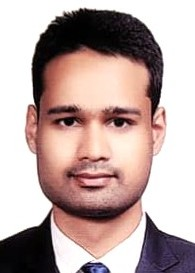
\includegraphics[width=1in,height=1.25in,clip,keepaspectratio]{bio_images/tiv.jpeg}}]{Tivranshu}
received the B.Tech. (CSE) degree from Guru Gobind Singh Indraprastha University, Delhi, India. He is currently pursuing the Integrated Ph.D. (IT) degree at the Indian Institute of Information Technology, Allahabad, India. His research interests include wireless sensor networks, unmanned aerial vehicles, and the Internet of Things.
\end{IEEEbiography}
\vspace{-2em}


\begin{IEEEbiography}[{
\includegraphics[width=1in,height=1.25in,clip,keepaspectratio]{bio_images/Kushagra_Gupta.jpeg}}]{Kushagra Gupta}
is currently pursuing the B.Tech. (IT) degree at the Indian Institute of Information Technology, Allahabad, India. His research interests include wireless sensor networks, unmanned aerial vehicles, and the Internet of Things.
\end{IEEEbiography}
\vspace{-2em}

\begin{IEEEbiography}[{
\includegraphics[width=1in,height=1.25in,clip,keepaspectratio]{bio_images/shivam_img.jpg.jpeg}}]{Shivam Chaturvedi}
is currently pursuing the B.Tech. (IT) degree at the Indian Institute of Information Technology, Allahabad, India. His research interests include wireless sensor networks, unmanned aerial vehicles, and the Internet of Things.
\end{IEEEbiography}
\vspace{-2em}

\begin{IEEEbiography}[{
\includegraphics[width=1in,height=1.25in,clip,keepaspectratio]{bio_images/tanmay.jpeg}}]{Tanmay Mathurvaishya}
is currently pursuing the B.Tech. (IT) degree at the Indian Institute of Information Technology, Allahabad, India. His research interests include wireless sensor networks, unmanned aerial vehicles, and the Internet of Things.
\end{IEEEbiography}
\vspace{-2em}

\begin{IEEEbiography}[{
\includegraphics[width=1in,height=1.25in,clip,keepaspectratio]{bio_images/Nabajyoti.png}}]{Nabajyoti Mazumdar}
(Member, IEEE) received the M.Tech. and Ph.D. degrees from the Indian Institute of Technology (ISM), Dhanbad. He is currently an Assistant Professor with the Department of Information Technology, Indian Institute of Information Technology, Allahabad, India. His research focuses on wireless sensor networks, the Internet of Things (IoT), and soft computing techniques.
\end{IEEEbiography}




\end{document}
